%%%%%%%%%%%%%%%%%%%%%%%%%%%%%%%%%%%%%%%%%
% Masters/Doctoral Thesis 
% LaTeX Template
% Version 1.43 (17/5/14)
%
% This template has been downloaded from:
% http://www.LaTeXTemplates.com
%
% Shahab SHARIAT BAGHERI 
%\subsection http://users.ecs.soton.ac.uk/srg/softwaretools/document/templates/
% and
% Sunil Patel
% http://www.sunilpatel.co.uk/thesis-template/
%
% License:
% CC BY-NC-SA 3.0 (http://creativecommons.org/licenses/by-nc-sa/3.0/)
%
% Note:
% Make sure to edit document variables in the Thesis.cls file
%
%%%%%%%%%%%%%%%%%%%%%%%%%%%%%%%%%%%%%%%%%

%----------------------------------------------------------------------------------------
%	PACKAGES AND OTHER DOCUMENT CONFIGURATIONS
%----------------------------------------------------------------------------------------

\documentclass[11pt, oneside]{Thesis} % The default font size and one-sided printing (no margin offsets)

\graphicspath{{Pictures/}} % Specifies the directory where pictures are stored

\usepackage{tikz}
\usepackage[square, numbers, comma, sort&compress]{natbib} % Use the natbib reference package - read up on this to edit the reference style; if you want text (e.g. Smith et al., 2012) for the in-text references (instead of numbers), remove 'numbers' 
\usepackage{caption}
\usepackage{subcaption}
\usepackage{float}
% table sizing
\usepackage{adjustbox}
\usepackage{graphicx}
\usepackage{placeins}
\usepackage{listings}
%%%
\usepackage{schemabloc}
\usetikzlibrary{circuits}
%%%

\usetikzlibrary{arrows,positioning,shapes,snakes}

%%%
\DeclareMathAlphabet{\mathpzc}{OT1}{pzc}{m}{it}
\newcommand{\z}{\mathpzc{z}}
%%%

\hypersetup{urlcolor=blue, colorlinks=true} % Colors hyperlinks in blue - change to black if annoying
\title{\ttitle} % Defines the thesis title - don't touch this

\lstset{
  language=python,
  basicstyle=\small,
  breaklines=true
  }


\begin{document}

\frontmatter % Use roman page numbering style (i, ii, iii, iv...) for the pre-content pages

\setstretch{1.3} % Line spacing of 1.3

% Define the page headers using the FancyHdr package and set up for one-sided printing
\fancyhead{} % Clears all page headers and footers
\rhead{\thepage} % Sets the right side header to show the page number
\lhead{} % Clears the left side page header

\pagestyle{fancy} % Finally, use the "fancy" page style to implement the FancyHdr headers

\newcommand{\suma}{\Large$+$}
\newcommand{\inte}{$\displaystyle \int$}
\newcommand{\derv}{\huge$\frac{d}{dt}$}
\newcommand{\HRule}{\rule{\linewidth}{0.5mm}} % New command to make the lines in the title page

% PDF meta-data
\hypersetup{pdftitle={\ttitle}}
\hypersetup{pdfsubject=\subjectname}
\hypersetup{pdfauthor=\authornames}
\hypersetup{pdfkeywords=\keywordnames}

%----------------------------------------------------------------------------------------
%	TITLE PAGE
%----------------------------------------------------------------------------------------

\begin{titlepage}

\begin{center}
 
\includegraphics[width=0.15\textwidth,natwidth=610,natheight=642]{telecom.jpeg}
 
\includegraphics[width=0.3\textwidth,natwidth=610,natheight=642]{cisco.png}

\textsc{\LARGE Paris Saclay University and TELECOM ParisTech}\\[1.5cm] % University name
\textsc{\Large Internship report \\ Master of Multimedia Networking} % Thesis type

\HRule \\[0.2cm] % Horizontal line
{\huge \bfseries \ttitle}\\[0.4cm] % Thesis title
\HRule \\[1.2cm] % Horizontal line


\begin{minipage}{0.4\textwidth}

\begin{flushleft} \large
\emph{Author:}\\
{\authornames} % Author name - remove the \href bracket to remove the link
\end{flushleft}
\end{minipage}
\begin{minipage}{0.4\textwidth}

\begin{flushright} \large
\emph{Responsbile of Internship:}\\
\href{https://scholar.google.com/citations?user=Q36qUAsAAAAJ&hl=fr}{Luca MUSCARIELLO}\\
% Supervisor name - remove the \href bracket to remove the link  
\end{flushright}

\end{minipage}\\[1.8cm]
%\degreename\\[0.5cm] % University requirement text


%\textit\\{in the}[0.4cm]

%\deptname\\[0.5cm] % Research group name and department name



{\large \today}
\vfill
\end{center}

\end{titlepage}

%----------------------------------------------------------------------------------------
%	DECLARATION PAGE
%	Your institution may give you a different text to place here
%----------------------------------------------------------------------------------------

%\Declaration{
%
%\addtocontents{toc}{\vspace{1em}} % Add a gap in the Contents, for aesthetics
%
%I, \authornames, declare that this thesis titled, '\ttitle' and the work presented in it are my own. I confirm that:
%
%\begin{itemize} 
%\item[\tiny{$\blacksquare$}] This work was done wholly or mainly while in candidature for a research degree at this University.
%\item[\tiny{$\blacksquare$}] Where any part of this thesis has previously been submitted for a degree or any other qualification at this University or any other institution, this has been clearly stated.
%\item[\tiny{$\blacksquare$}] Where I have consulted the published work of others, this is always clearly attributed.
%\item[\tiny{$\blacksquare$}] Where I have quoted from the work of others, the source is always given. With the exception of such quotations, this thesis is entirely my own work.
%\item[\tiny{$\blacksquare$}] I have acknowledged all main sources of help.
%\item[\tiny{$\blacksquare$}] Where the thesis is based on work done by myself jointly with others, I have made clear exactly what was done by others and what I have contributed myself.\\
%\end{itemize}
% 
%Signed:\\
%\rule[1em]{25em}{0.5pt} % This prints a line for the signature
% 
%Date:\\
%\rule[1em]{25em}{0.5pt} % This prints a line to write the date
%}
%
%\clearpage % Start a new page

%----------------------------------------------------------------------------------------
%	QUOTATION PAGE
%----------------------------------------------------------------------------------------

\pagestyle{empty} % No headers or footers for the following pages

\null\vfill % Add some space to move the quote down the page a bit

\textit{Learn from yesterday, live for today, hope for tomorrow. The important thing is not to stop Questioning.}

\begin{flushright}
Albert Einstein
\end{flushright}

\vfill\vfill\vfill\vfill\vfill\vfill\null % Add some space at the bottom to position the quote just right

\clearpage % Start a new page

%----------------------------------------------------------------------------------------
%	ABSTRACT PAGE
%----------------------------------------------------------------------------------------

\addtotoc{Abstract} % Add the "Abstract" page entry to the Contents

\abstract % Add a gap in the Contents, for aesthetics
\textbf{I}nformation \textbf{C}entric \textbf{N}etworking (ICN) in one sentence is rethinking of internet in the sense that it will be no more calling (IP-architecutre) for communication rather we search the content on the network using caching data with different on each node. Notably this architecture is a good suite for embedded systems in which you have good control on caching level , memory allocations, network functionalities. In this case like all networks in each node your packets need routing table to send. In this work we propose 4 different strategies called \textit{TreeOnConsumer}, \textit{TreeOnProducer}, \textit{MinCostMultipath}, \textit{MaxFlow} which decide the best path to create faces through proper interfaces then forward packets. Finally we design an algorithm to automatize the algorithm to be chosen in function of network conditions. We developed \textit{Lurch}, the emulator to interact with linux containers dynamically on cisco's server. We use \textit{ndn-icp-download} an application for downloading ndn content. We use \textit{ifstat} linux utility to read network interface statistics.  
Results are real data rate packet in Kbps using these algorithms which choose different paths according to proper algorithm and network condition.

%\clearpage % Start a new page

%----------------------------------------------------------------------------------------
%	ACKNOWLEDGEMENTS
%----------------------------------------------------------------------------------------

\setstretch{1.3} % Reset the line-spacing to 1.3 for body text (if it has changed)
%
%\acknowledgements{\addtocontents{toc}{\vspace{1em}} % Add a gap in the Contents, for aesthetics
%%%
%%%Thanks to my solid academic Internship, today I can write rapidly several programs and models in Communications Systems \ldots
%%}
\clearpage % Start a new page

%----------------------------------------------------------------------------------------
%	LIST OF CONTENTS/FIGURES/TABLES PAGES
%----------------------------------------------------------------------------------------

\pagestyle{fancy} % The page style headers have been "empty" all this time, now use the "fancy" headers as defined before to bring them back

\lhead{\emph{Contents}} % Set the left side page header to "Contents"
\tableofcontents % Write out the Table of Contents

\lhead{\emph{List of Figures}} % Set the left side page header to "List of Figures"
\listoffigures % Write out the List of Figures

\lhead{\emph{List of Tables}} % Set the left side page header to "List of Tables"
%\listoftables % Write out the List of Tables

%----------------------------------------------------------------------------------------
%	ABBREVIATIONS
%----------------------------------------------------------------------------------------

%\clearpage % Start a new page
%%
%\setstretch{1.5} % Set the line spacing to 1.5, this makes the following tables easier to read
%%
%\lhead{\emph{Abbreviations}} % Set the left side page header to "Abbreviations"
%\listofsymbols{ll} % Include a list of Abbreviations (a table of two columns)
%%{
%\textbf{CPFSK} & \textbf{C}ontinous \textbf{P}hase \textbf{F}requency \textbf{S}hit \textbf{K}eying \\
%
%\textbf{BFSK} & \textbf{B}inary \textbf{F}requency \textbf{S}hit \textbf{K}eying \\
%%
%\textbf{GFSK} & \textbf{G}aussian \textbf{F}requency \textbf{S}hit \textbf{K}eying \\
%\textbf{DASH7} & \textbf{D}evelopers \textbf{A}lliance for \textbf{S}tandard \textbf{H}armonization
%\textbf{Acronym} & \textbf{W}hat (it) \textbf{S}tands \textbf{F}or \\
%}

%----------------------------------------------------------------------------------------
%	PHYSICAL CONSTANTS/OTHER DEFINITIONS
%----------------------------------------------------------------------------------------

\texttt{%\clearpage % Start a new page
%
%\lhead{\emph{Physical Constants}} % Set the left side page header to "Physical Constants"
%
%\listofconstants{lrcl} % Include a list of Physical Constants (a four column table)
{
%Speed of Light & $c$ & $=$ & $2.997\ 924\ 58\times10^{8}\ \mbox{ms}^{-\mbox{s}}$ (exact)\\
%% Constant Name & Symbol & = & Constant Value (with units) \\
}}

%----------------------------------------------------------------------------------------
%	SYMBOLS
%----------------------------------------------------------------------------------------

%\clearpage % Start a new page
%
%\lhead{\emph{Symbols}} % Set the left side page header to "Symbols"
%
%\listofnomenclature{lll} % Include a list of Symbols (a three column table)
{
%$a$ & distance & m \\
%$P$ & power & W (Js$^{-1}$) \\
% Symbol & Name & Unit \\

%& & \\ % Gap to separate the Roman symbols from the Greek

%$\omega$ & angular frequency & rads$^{-1}$ \\
% Symbol & Name & Unit \\
}

%----------------------------------------------------------------------------------------
%	DEDICATION
%----------------------------------------------------------------------------------------

\setstretch{1.3} % Return the line spacing back to 1.3

\pagestyle{empty} % Page style needs to be empty for this page

\dedicatory{To \textit{My Parents} and \textit{PIRL} \ldots} % Dedication text

\addtocontents{toc}{\vspace{2em}} % Add a gap in the Contents, for aesthetics

%----------------------------------------------------------------------------------------
%	THESIS CONTENT - CHAPTERS
%----------------------------------------------------------------------------------------

\mainmatter % Begin numeric (1,2,3...) page numbering

\pagestyle{fancy} % Return the page headers back to the "fancy" style

% Include the chapters of the thesis as separate files from the Chapters folder
% Uncomment the lines as you write the chapters

% Chapter 1

\chapter{Introduction} % Main chapter title

\label{Chapter1} % For referencing the chapter elsewhere, use \ref{Chapter1} 

\lhead{Chapter 1. \emph{Introduction}} % This is for the header on each page - perhaps a shortened title

%----------------------------------------------------------------------------------------
\section{Named Data Networking}

Today's Internet's hourglass architecture centers on a
universal network layer (i.e., IP) which implements the minimal functionality  necessary  for  global interconnectivity. This thin  waist  enabled  the Internet's  explosive  growth  by  allowing both lower and upper layer technologies to innovate independently.  However, IP was designed to create a communication  network
, where  packets  named  only  communication endpoints.  Sustained growth in e-commerce, digital media, social networking, and smartphone applications has led to dominant use of the Internet as a distribution network.

Distribution networks are more general than communication
networks, and solving distribution problems via a point to point communication protocol is complex and error-prone.
Named Data Networking (NDN) project proposed an
evolution of the IP architecture that generalizes the role of this  thin  waist,  such  that  packets  can  name  objects  rather than  communication  endpoint.

\section{PIRL}

My internship has been held in CICSO Company and i had a great pleasure to be under direction of Cisco Principle Engineer Luca MUSCARIELLO  for this period of 6 months. PIRL is acrynom for \textbf{P}aris \textbf{I}nnovation and \textbf{R}esearch \textbf{L}ab which is located in Issy les moulineaux region, near to Paris (\ref{cisco}). Leader of ICN in PIRL is Giovanna CAROFIGLIO. Alain FIOCCO is the  Director CTO of PIRL.


\begin{figure}

\begin{center}

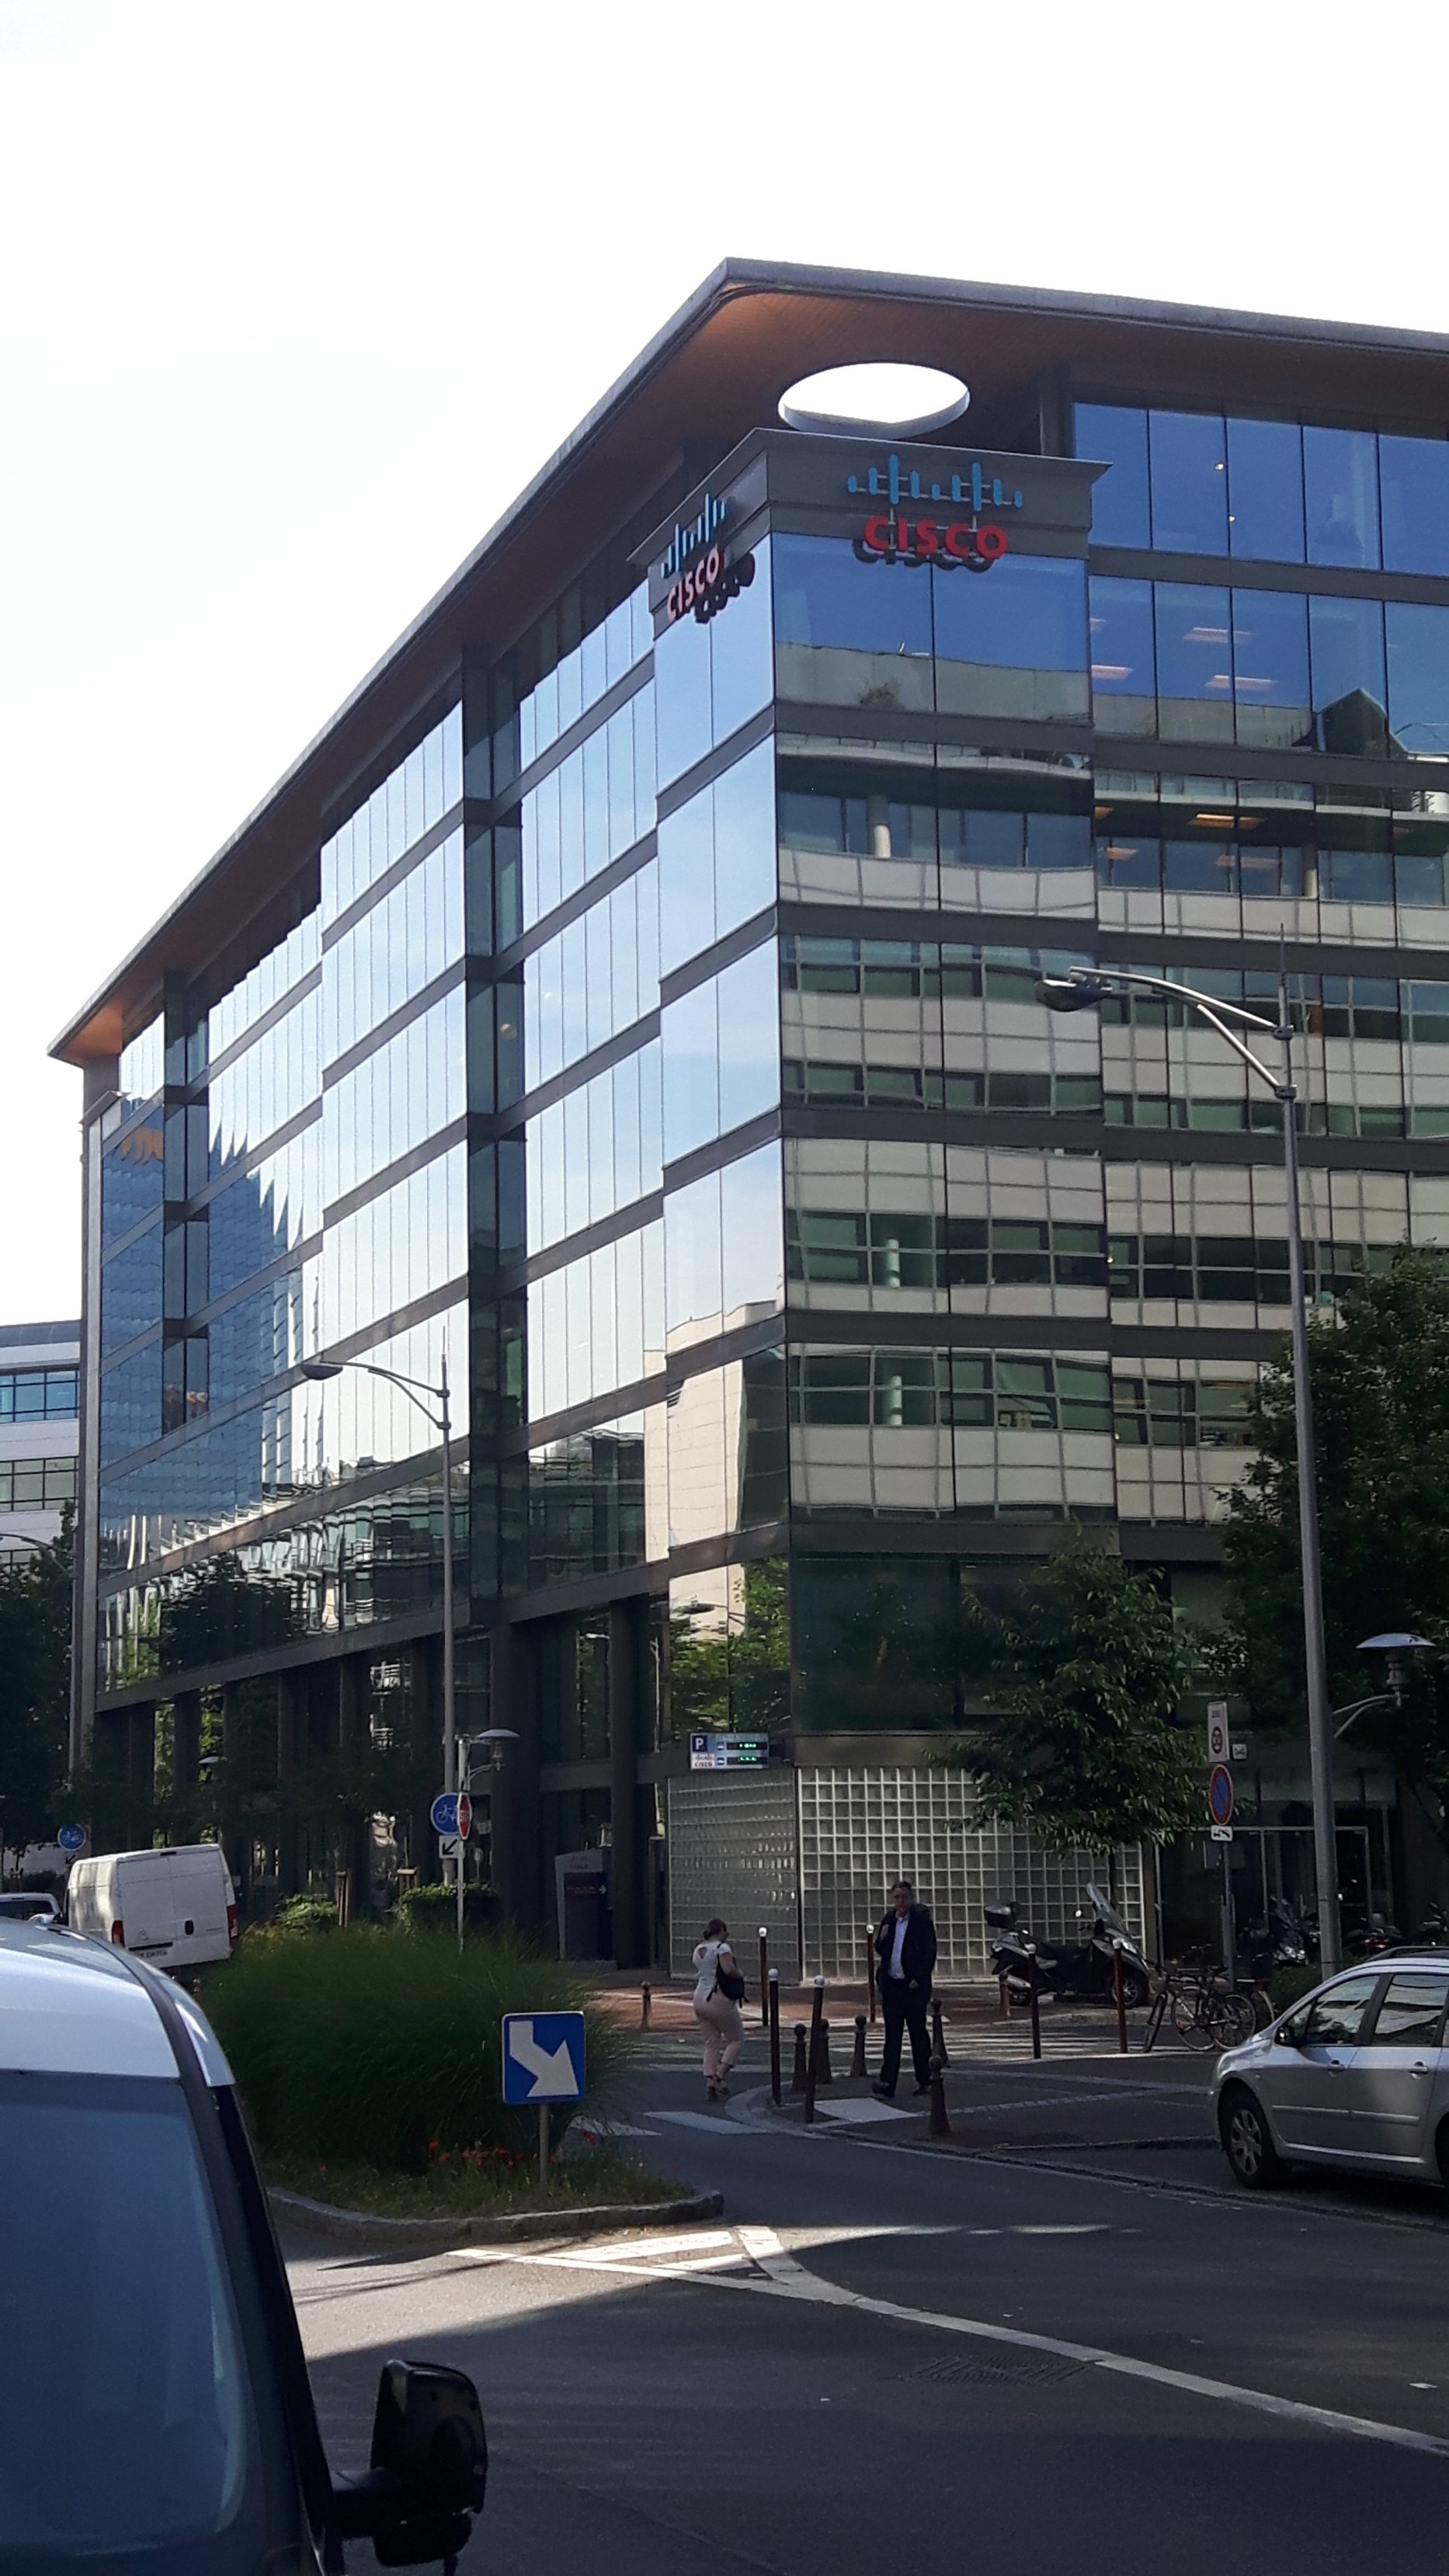
\includegraphics[scale = 0.1]{Pictures/cisco.jpg}

\caption{Cisco Systems France - 9h:40, 22 July 2016} \label{cisco} 

\end{center}

\end{figure}


\section{Tools of Internship}

I used a machine with an operating system of the latest distribution of Linux Ubuntu 16.04, lenovo ThinkPad Laptop serie T450 of CORE i5 with 2 cores. Our expermimental tests are totally done on powerful cisco's server (pirl-ndn-2.com) with 48 cores and 252 GB memory RAM. We have used \textit{ifstat} of linux implementation to see the rates output of result and \textit{ndn-icp-download} application to downloading in MultiThreading processing on different containers at the same time. Latest version of Python (3.5) was used to compile the program.

\textbf{\Huge{Lurch}} is an orchestrator for large scale and highly reconfigurable NDN experimental test-beds written in python for any platform, i.e., large Grids, local lab, providing connectivity among servers involved in the test-bed, ... .

Basically Python language is perfectly designed to develop new algorithms becasue of it's very usefull functionalities and handfull algorithm sense, I mean you can write a 10 lines of C code in just one line in python! Albeit according to \cite{python} we note that Python implementations may be not as fast as C/C++ counterparts but they scale with the input size according to the theory which claims a good reason to choose \textit{Python} anyway as the core part of Lurch.

Actually this emulator emulates linux containers which are like virtual machines in function of your setup. I said like, becasue there is difference between VMs and containers and the difference is the overhead that comes with running a separate kernel and simulating all the hardware when we have VMs. These containers are produced by ubuntu image server installed on the server then \textit{Lurch} clone this image to different machines to have virtual network machines. 

This tool can be used for researchers to test their customized network on the real virtual machines and run some usefull experiments. This means you can have your own OpenFlow who enables network controller to determine the path of network packets across a network of switches or virtual ethernet interfaces (MACVLAN interfaces).

Lurch produces some Modules in which you can setup your network: \textit{NDNmanager}, \textit{MobilityManager}, \textit{Topology}, \textit{Clustermanager}. We added a new Module Called \textit{RoutingNDN} in which you will find different algorithms to choose and some functionalities for modifying the Graph of network.
We also added some new functionalities on \textit{CommandLineInterface}, \textit{NetworkManager}, \textit{ConfigReader} and \textit{NDNmanager} module to have the ability to change the network parameters like capacity, delay, forwarding plane instantly which was very important in our testing experiments.

Figure \ref{cli} shows configuration, setup step of Lurch.
'../Network' is the address of input configuration files like Topology, position of Clients and Producers and the content that they search, mobility model of network a setting file about URL server, layer2 protocols, information about mobility parameteres, ... . By this way you can make your clusters on server.

$m942$ is ExperimentID of the user who runs his expermiment on this server. We use SSH remote login service to enter to each containers.

\begin{figure}[H]

\begin{center}

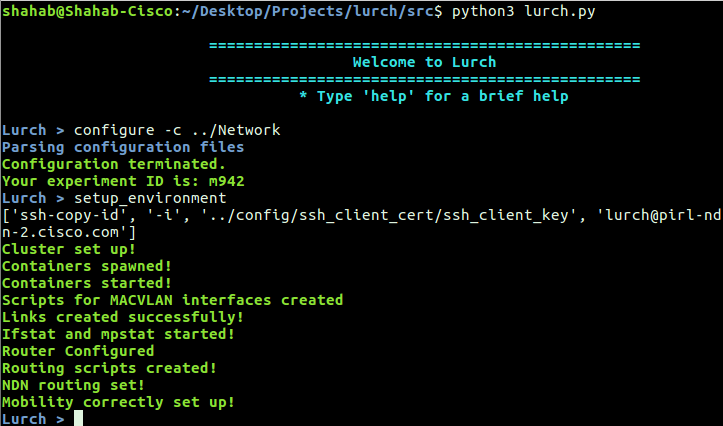
\includegraphics[scale = 0.35]{Pictures/lurch.png}

\caption{Command Line Interface} \label{cli} 

\end{center}

\end{figure}

 
Figure \ref{table} is the table of linux containers running on the server \textit{pirl-ndn-2.com}. You can see the IPv4 virtual interfaces on each container and the name NodeID for each interfaces which have the same as NodeID of end link. On Container \textit{m942michel} you see a \textit{wlan0} interface becasue this node is choosen Access Point node in setup level. This interface is now eumulated by ndnSIM using lxc-wifi-tap script. In figure \ref{data} you can see an example of how we can get our output in Kbps for each link.


\begin{figure}[H]

\begin{center}

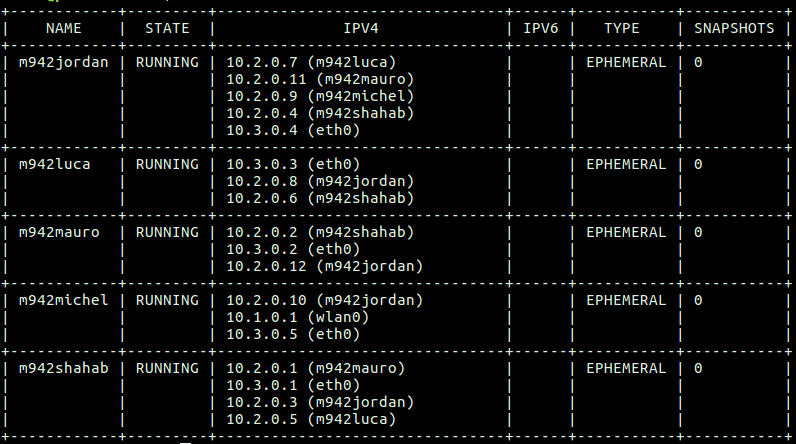
\includegraphics[scale = 0.3]{Pictures/table.png}

\caption{Table of Emulated Linux Containers on pirl-ndn-2.com} \label{table} 

\end{center}

\end{figure}


 
\textit{setup environment} will setup completely your containers on the server with all of information needed to have a virtual network. As figure \ref{cli} shows step by step setups which are successful which is not quiet short! \textit{Routing scripts created} is where the routing scritps are creating in each different containers then you have \textit{NDN routing set} step when you push your scripts on containers. normally this stage takes more time than the previous step. Each routing scripts includes bash commands to run which are coming from NFD command line interfaces (Picture \ref{script}). By \textit{create} and  command you can create a new face and \textit{register} you can add the routes in the RIB.   
 
\begin{figure}[H]

\begin{center}

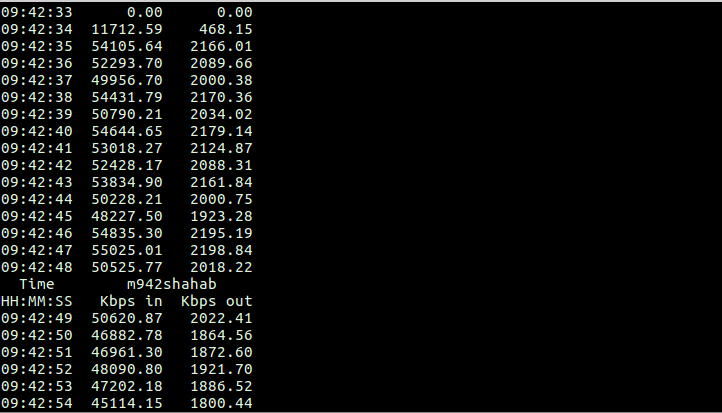
\includegraphics[scale = 0.35]{Pictures/data.png}

\caption{Rates Trace using ifstat} \label{data} 

\end{center}

\end{figure}
 
 
 
Next step to continue is doing \textit{start repo} command line which creates a dameon of \textit{repo-ng} application on all producer nodes NFD using a timer which waits for state of process intelligently. Figure \ref{repo} shows this step in Lurch. As you can see it declares you on which node the repository is created and how many repositories exist on the network.



\begin{figure}[H]

\begin{center}

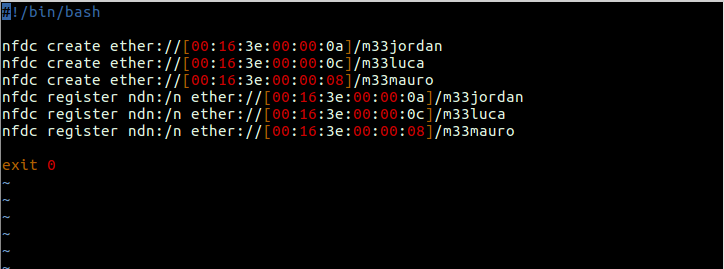
\includegraphics[scale = 0.35]{Pictures/script.png}

\caption{NDN Routing Script} \label{script} 

\end{center}

\end{figure}


\begin{figure}[H]

\begin{center}

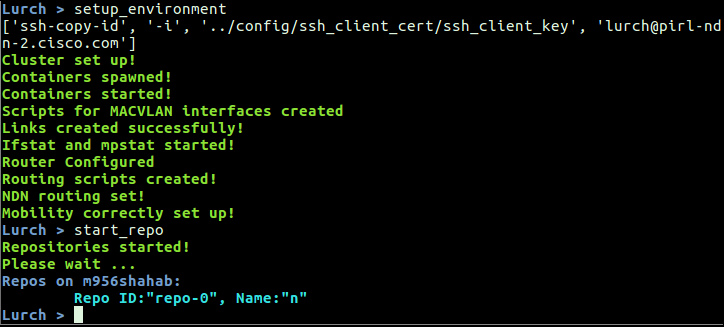
\includegraphics[scale = 0.35]{Pictures/start_repo.png}

\caption{Starting Repository Daemon} \label{repo} 

\end{center}

\end{figure}




In figure \ref{download} you can see by \textit{list client} and \textit{list repo} command line which lists the clients and producers on your network. Then as we have started repositories engine, now it's time to choose the routing algorithm. It's easy, you just write route set, then TAB to see the different algorithms which will appear on your terminal, then you can select one of them and click ENTER.

Now it's time to run your experiment, this is doing just by \textit{start} command line you can see 2 downloading thread is started at the same time becasue you had 2 clients searching same content.  

\begin{figure}[H]

\begin{center}

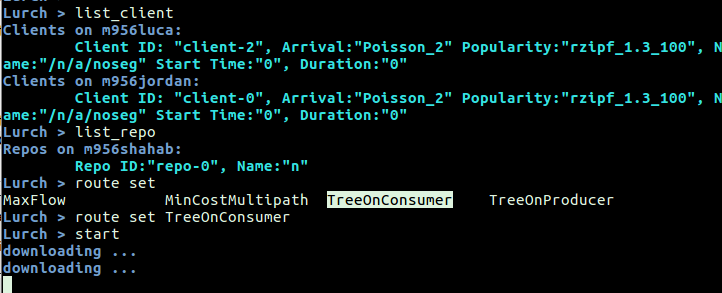
\includegraphics[scale = 0.35]{Pictures/download.png}

\caption{Downloading Step} \label{download} 

\end{center}

\end{figure}


In figure \ref{capacity} by \textit{link show} command you can see all of link capacities. by \textit{link edit shahab jordan 20000} you can change link capacity between 'shahab' and 'luca' container.

\begin{figure}[H]

\begin{center}

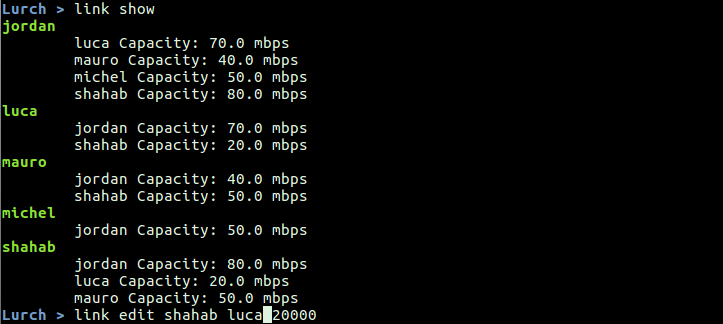
\includegraphics[scale = 0.55]{Pictures/capacity.png}

\caption{Link Capacity Modification} \label{capacity} 

\end{center}

\end{figure}
 
We have implemented also implemented an algorithm to full automatization the routing, it means that in function of network situation you can adapt proper algorithm to your routing updates, which depend on workload system can be varried and played. This can be very usefull when we want to have demonstrations on our work.

Picture \ref{auto} shows well when we do \textit{route auto} TreeOnConsumer algorithm is chosen becasue of the structure of workload. It means that in workload you have one producer and 2 consumers who are searching the content. So this algorithm is just a brain who understands and can adapt algorithms to proper station of system.

\begin{figure}[H]

\begin{center}

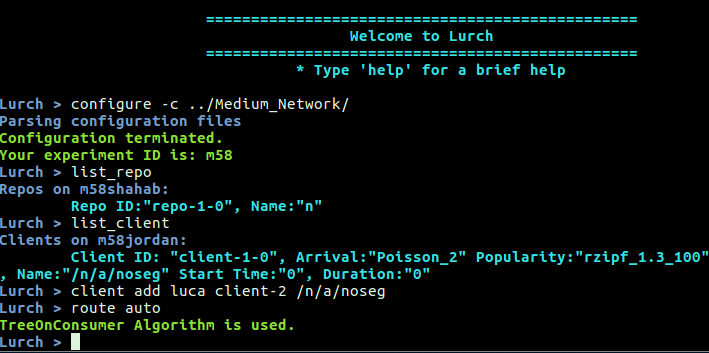
\includegraphics[scale = 0.35]{Pictures/auto.png}

\caption{Automatization algorithm} \label{auto} 

\end{center}

\end{figure}


In figure \ref{lxc} you can see the difference between linux containers and virtual machines which is very important. Actually linux containers use \textit{cgroups} kernel module to get prior for each machine on the same host server.

This appearance makes linux containers to be very successful becasue of ability to manage and control the guests machines becasue basically they share one kernel on machine. 

\begin{figure}[H]

\begin{center}

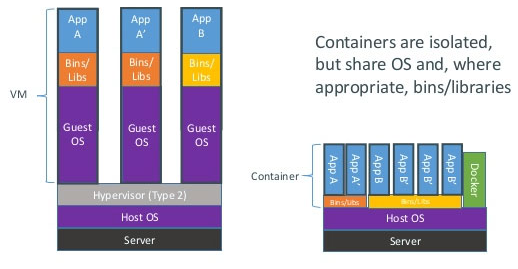
\includegraphics[scale = 0.35]{Pictures/lxc.png}

\caption{Linux Containers vs Virtual Machines} \label{lxc} 

\end{center}

\end{figure}


 
\section{Scope and Objectives}
In These days, 2016,  there is a lot of research and new ideas on 5G cellular networks on different aspects of Research and Development from advanced chip designing techniques and hardware, antenna designing to whole different network architectures, algorithms, computations even some ideas to combine it with Quad drones robots and ... for the 2020 plan. It's a bit like the evolution from 1999 to 2000 for IT and computer science domain.

ICN has a fundamental designing philosophy in which you will be able to have like a PeerToPeer (Figure \ref{peertopeer}) or IoT way of thinking in which each node will be a peer who can talk with his neighbours using P2P protocol on second layer of ICN model where he is searching chunk of your data as it's clear on the waist ICN Model (Figure \ref{spec}). 


\begin{figure}[H]

\begin{center}

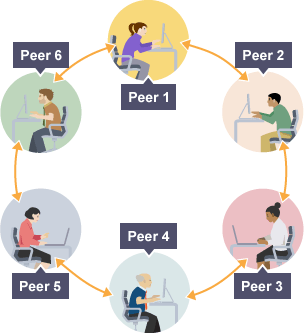
\includegraphics[scale = 0.4]{Pictures/peertopeer.png}

\caption{PeerToPeer Network} \label{peertopeer} 

\end{center}

\end{figure}



Information Centric Networking layer model shows a bit names in ICN can be like a replacement in TCP/IP architecure in this sense you can imagine that all nodes have the same responsibility to pipline packets to the network and you can have Device 2 Device (D2D) communication in which instead of putting clock at a special time alarm in each night, Or at the evening, light and heat of Sunshine (with embedded Sensor installed on window) can capture temperature of heatness then talk to your Table-Lamp installed beside your bedroom and turn it on and your alarm clock to ring and waking you up or immediately turn your microwave on to heat bread inside (\ref{internetofthings})



\begin{figure}[H]

\begin{center}

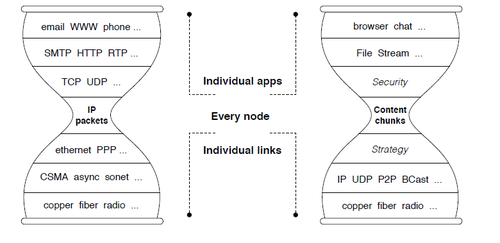
\includegraphics[scale = 0.6]{Pictures/spec.png}

\caption{ICN vs TCP/IP OSI model} \label{spec} 

\end{center}

\end{figure}

\begin{figure}[H]

\begin{center}

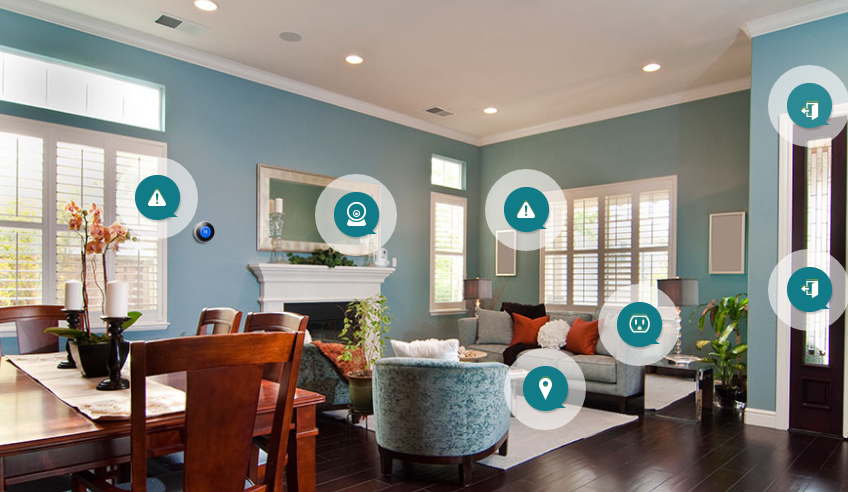
\includegraphics[scale = 0.35]{Pictures/internetofthings.png}

\caption{Smart Room in IoT} \label{internetofthings} 

\end{center}

\end{figure}

Figure \ref{2020} estimation calculated shows more than 25 Billion things will be connected in 2020! \textit{Smart Cities} is another word that we hear everywhere in Technology domain in these days. So it sounds there exists a strong merging between communicaiton world and computer/artificial intelligence or robotics. This merging needs a better solution for communicating between machines/robots. We believe that ICN is a good architecture to solve this essential problem. It seems also more and more calling communication system philosophy is \textit{expired}! or if it is not today it will be expired in near future. ICN as Jacobson et al explained in \cite{jacobson} has more intelligent and logic architecture.


\begin{figure}[H]

\begin{center}

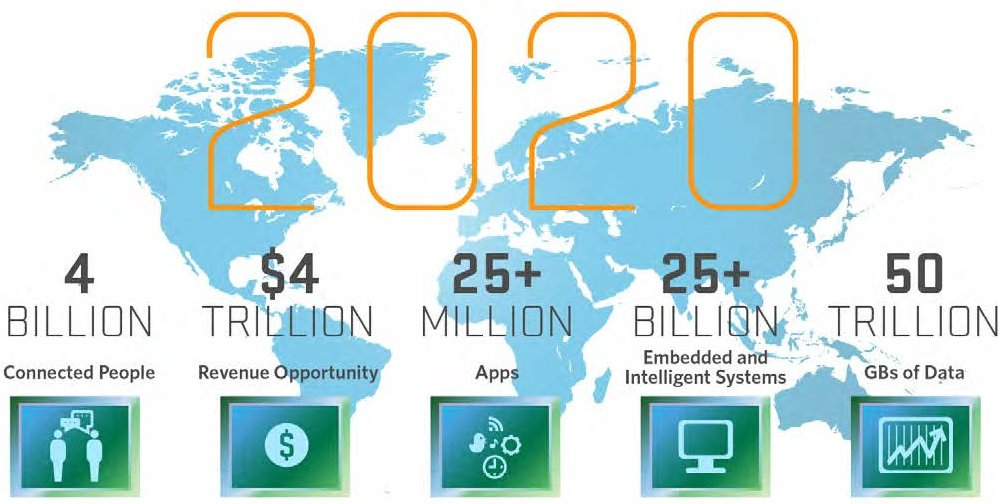
\includegraphics[scale = 0.31]{Pictures/2020.jpg}

\caption{Plan 2020} \label{2020} 

\end{center}

\end{figure}


 We beleive ICN architecture can be a very suitable fit for 5G networks becasue of its advantage against TCP/IP architecture, and important network functionalities like congestion control, storage data, security, and mobility protocols which can be a good idea specially in case of wireless mobile communication in which nodes can be moved with every speed and channel conditions in the case that all of objects are connected together and they talk together with ICN protocol specification.

So if you are in Cisco Systems Paris and you search \textit{'movie.mp4'} on YouTube maybe on the network one of your neighbours has been downloaded once. So now instead of talking with YouTube's server in USA you can take it from one of your near nodes beside Issy val de seine train station and not making more extra traffic on network.


In this way Cisco has been investigated ICN in context of 5G and notably for popular applications like video delivery, which is one of the most popular applications in these days, people want to see a video on YouTube, Netflix, ... everywhere and everytime in the metro stations, in the building, in the bitches with different Transcoder of video coding and with the highest speed of downloading which network should produce them.

\textit{Four Routing} algorithms (Strategies) are added to \textit{Lurch} to use in different conditions of Network. \textit{Auto} strategy also is added which is as an algorithm that chooses the proper strategy in function of network condition and in demand of clients. This strategy is added on \textit{NetworkManager} Module.








%
%\section{Physical Layer}
%In this chapter , at first, we are going to explain about the kinds of channels which is used in DASH7 Protocl which in that we are showing the power spectral density for different channels and our Masks definition. 
%If you are familiar with \LaTeX{}, then you can familiarise yourself with the contents of the Zip file and the directory structure and then place your own information into the `\texttt{Thesis.cls}' file. Section \ref{FillingFile} on page \pageref{FillingFile} tells you how to do this. Make sure you read section \ref{ThesisConventions} about thesis conventions to get the most out of this template and then get started with the `\texttt{Thesis.tex}' file straightaway.
%
%If you are new to \LaTeX{} it is recommended that you carry on reading through the rest of the information in this document.
%
%\subsection{Spectrum Utilization and Channels}
%
%This \LaTeX{} Thesis Template is originally based and created around a \LaTeX{} style file created by Steve R.\ Gunn from the University of Southampton (UK), department of Electronics and Computer Science. You can find his original thesis style file at his site, here:\\
%\href{http://www.ecs.soton.ac.uk/~srg/softwaretools/document/templates/}{\texttt{http://www.ecs.soton.ac.uk/$\sim$srg/softwaretools/document/templates/}}
%
%My thesis originally used the `\texttt{ecsthesis.cls}' from his list of styles. However, I knew \LaTeX{} could still format better. To get the look I wanted, I modified his style and also created a skeleton framework and folder structure to place the thesis files in.
%
%This Thesis Template consists of that modified style, the framework and the folder structure. All the work that has gone into the preparation and groundwork means that all you have to bother about is the writing.
%Before you begin using this template you should ensure that its style complies with the thesis style guidelines imposed by your institution. In most cases this template style and layout will be suitable. If it is not, it may only require a small change to bring the template in line with your institution's recommendations.
%
%%----------------------------------------------------------------------------------------
%
%\section{What this Template Includes}
%
%\subsection{Folders}
%
%This template comes as a single Zip file that expands out to many files and folders. The folder names are mostly self-explanatory:
%
%\textbf{Appendices} -- this is the folder where you put the appendices. Each appendix should go into its own separate `\texttt{.tex}' file. A template is included in the directory.
%
%\textbf{Chapters} -- this is the folder where you put the thesis chapters. A thesis usually has about seven chapters, though there is no hard rule on this. Each chapter should go in its own separate `\texttt{.tex}' file and they usually are split as:
%\begin{itemize}
%\item Chapter 1: Introduction to the thesis topic
%\item Chapter 2: Background information and theory
%\item Chapter 3: (Laboratory) experimental setup
%\item Chapter 4: Details of experiment 1
%\item Chapter 5: Details of experiment 2
%\item Chapter 6: Discussion of the experimental results
%\item Chapter 7: Conclusion and future directions
%\end{itemize}
%This chapter layout is specialised for the experimental sciences.
%
%\textbf{Figures} -- this folder contains all figures for the thesis. These are the final images that will go into the thesis document.
%
%\textbf{Primitives} -- this is the folder that contains scraps, particularly because one final image in the `Figures' folder may be made from many separate images and photos, these source images go here. This keeps the intermediate files separate from the final thesis figures.
%
%\subsection{Files}
%
%Included are also several files, most of them are plain text and you can see their contents in a text editor. Luckily, many of them are auxiliary files created by \LaTeX{} or BibTeX and which you don't need to bother about:
%
%\textbf{Bibliography.bib} -- this is an important file that contains all the bibliographic information and references that you will be citing in the thesis for use with BibTeX. You can write it manually, but there are reference manager programs available that will create and manage it for you. Bibliographies in \LaTeX{} are a large subject and you may need to read about BibTeX before starting with this.
%
%\textbf{Thesis.cls} -- this is an important file. It is the style file that tells \LaTeX{} how to format the thesis. You will also need to open this file in a text editor and fill in your own information (such as name, department, institution). Luckily, this is not too difficult and is explained in section \ref{FillingFile} on page \pageref{FillingFile}.
%
%\textbf{Thesis.pdf} -- this is your beautifully typeset thesis (in the PDF file format) created by \LaTeX{}.
%
%\textbf{Thesis.tex} -- this is an important file. This is the file that you tell \LaTeX{} to compile to produce your thesis as a PDF file. It contains the framework and constructs that tell \LaTeX{} how to layout the thesis. It is heavily commented so you can read exactly what each line of code does and why it is there. After you put your own information into the `\texttt{Thesis.cls}' file, go to this file and begin filling it in -- you have now started your thesis!
%
%\textbf{vector.sty} -- this is a \LaTeX{} package, it tells \LaTeX{} how to typeset mathematical vectors. Using this package is very easy and you can read the documentation on the site (you just need to look at the `\texttt{vector.pdf}' file):\\
%\href{http://www.ctan.org/tex-archive/macros/latex/contrib/vector/}{\texttt{http://www.ctan.org/tex-archive/macros/latex/contrib/vector/}}
%
%\textbf{lstpatch.sty} -- this is a \LaTeX{} package required by this LaTeX template and is included as not all \TeX{} distributions have it installed by default. You do not need to modify this file.
%
%Files that are \emph{not} included, but are created by \LaTeX{} as auxiliary files include:
%
%\textbf{Thesis.aux} -- this is an auxiliary file generated by \LaTeX{}, if it is deleted \LaTeX{} simply regenerates it when you run the main `\texttt{.tex}' file.
%
%\textbf{Thesis.bbl} -- this is an auxiliary file generated by BibTeX, if it is deleted, BibTeX simply regenerates it when you run the main tex file. Whereas the `\texttt{.bib}' file contains all the references you have, this `\texttt{.bbl}' file contains the references you have actually cited in the thesis and is used to build the bibliography section of the thesis.
%
%\textbf{Thesis.blg} -- this is an auxiliary file generated by BibTeX, if it is deleted BibTeX simply regenerates it when you run the main `\texttt{.tex}' file.
%
%\textbf{Thesis.lof} -- this is an auxiliary file generated by \LaTeX{}, if it is deleted \LaTeX{} simply regenerates it when you run the main `\texttt{.tex}' file. It tells \LaTeX{} how to build the `List of Figures' section.
%
%\textbf{Thesis.log} -- this is an auxiliary file generated by \LaTeX{}, if it is deleted \LaTeX{} simply regenerates it when you run the main `\texttt{.tex}' file. It contains messages from \LaTeX{}, if you receive errors and warnings from \LaTeX{}, they will be in this `\texttt{.log}' file.
%
%\textbf{Thesis.lot} -- this is an auxiliary file generated by \LaTeX{}, if it is deleted \LaTeX{} simply regenerates it when you run the main `\texttt{.tex}' file. It tells \LaTeX{} how to build the `List of Tables' section.
%
%\textbf{Thesis.out} -- this is an auxiliary file generated by \LaTeX{}, if it is deleted \LaTeX{} simply regenerates it when you run the main `\texttt{.tex}' file.
%
%
%So from this long list, only the files with the `\texttt{.sty}', `\texttt{.bib}', `\texttt{.cls}' and `\texttt{.tex}' extensions are the most important ones. The other auxiliary files can be ignored or deleted as \LaTeX{} and BibTeX will regenerate them.
%
%%----------------------------------------------------------------------------------------
%
%\section{Filling in the `\texttt{Thesis.cls}' File}\label{FillingFile}
%
%You will need to personalise the thesis template and make it your own by filling in your own information. This is done by editing the `\texttt{Thesis.cls}' file in a text editor.
%
%Open the file and scroll down, past all the `$\backslash$\texttt{newcommand}\ldots' items until you see the entries for `\texttt{University Name}', `\texttt{Department Name}', etc\ldots.
%
%Fill out the information about your group and institution and ensure you keep to block capitals where it asks you to. You can also insert web links, if you do, make sure you use the full URL, including the `\texttt{http://}' for this.
%
%The last item you should need to fill in is the Faculty Name (in block capitals). When you have done this, save the file and recompile `\texttt{Thesis.tex}'. All the information you filled in should now be in the PDF, complete with web links. You can now begin your thesis proper!
%
%%----------------------------------------------------------------------------------------
%
%\section{The `\texttt{Thesis.tex}' File Explained}
%
%The \texttt{Thesis.tex} file contains the structure of the thesis. There are plenty of written comments that explain what pages, sections and formatting the \LaTeX{} code is creating. Initially there seems to be a lot of \LaTeX{} code, but this is all formatting, and it has all been taken care of so you don't have to do it.
%
%Begin by checking that your information on the title page is correct. For the thesis declaration, your institution may insist on something different than the text given. If this is the case, just replace what you see with what is required.
%
%Then comes a page which contains a funny quote. You can put your own, or quote your favourite scientist, author, person, etc\ldots Make sure to put the name of the person who you took the quote from.
%
%Next comes the acknowledgements. On this page, write about all the people who you wish to thank (not forgetting parents, partners and your advisor/supervisor).
%
%The contents pages, list of figures and tables are all taken care of for you and do not need to be manually created or edited. The next set of pages are optional and can be deleted since they are for a more technical thesis: insert a list of abbreviations you have used in the thesis, then a list of the physical constants and numbers you refer to and finally, a list of mathematical symbols used in any formulae. Making the effort to fill these tables means the reader has a one-stop place to refer to instead of searching the internet and references to try and find out what you meant by certain abbreviations or symbols.
%
%The list of symbols is split into the Roman and Greek alphabets. Whereas the abbreviations and symbols ought to be listed in alphabetical order (and this is \emph{not} done automatically for you) the list of physical constants should be grouped into similar themes.
%
%The next page contains a one line dedication. Who will you dedicate your thesis to?
%
%Finally, there is the section where the chapters are included. Uncomment the lines (delete the `\texttt{\%}' character) as you write the chapters. Each chapter should be written in its own file and put into the `Chapters' folder and named `\texttt{Chapter1}', `\texttt{Chapter2}, etc\ldots Similarly for the appendices, uncomment the lines as you need them. Each appendix should go into its own file and placed in the `Appendices' folder.
%
%After the preamble, chapters and appendices finally comes the bibliography. The bibliography style (called `\texttt{unsrtnat}') is used for the bibliography and is a fully featured style that will even include links to where the referenced paper can be found online. Do not under estimate how grateful you reader will be to find that a reference to a paper is just a click away. Of course, this relies on you putting the URL information into the BibTeX file in the first place.
%
%%----------------------------------------------------------------------------------------
%
%\section{Thesis Features and Conventions}\label{ThesisConventions}
%
%To get the best out of this template, there are a few conventions that you may want to follow.
%
%One of the most important (and most difficult) things to keep track of in such a long document as a thesis is consistency. Using certain conventions and ways of doing things (such as using a Todo list) makes the job easier. Of course, all of these are optional and you can adopt your own method.
%
%\subsection{Printing Format}
%
%This thesis template is designed for single sided printing as most theses are printed and bound this way. This means that the left margin is always wider than the right (for binding). Four out of five people will now judge the margins by eye and think, ``I never 
%noticed that before.''.
%
%The headers for the pages contain the page number on the right side (so it is easy to flick through to the page you want) and the chapter name on the left side.
%
%The text is set to 11 point and a line spacing of 1.3. Generally, it is much more readable to have a smaller text size and wider gap between the lines than it is to have a larger text size and smaller gap. Again, you can tune the text size and spacing should you want or need to. The text size can be set in the options for the `$\backslash$\texttt{documentclass}' command at the top of the `\texttt{Thesis.tex}' file and the spacing can be changed by setting a different value in the `$\backslash$\texttt{setstretch}' commands (scattered throughout the `\texttt{Thesis.tex}' file).
%
%\subsection{Using US Letter Paper}
%
%The paper size used in the template is A4, which is a common -- if not standard -- size in Europe. If you are using this thesis template elsewhere and particularly in the United States, then you may have to change the A4 paper size to the US Letter size. Unfortunately, this is not as simple as replacing instances of `\texttt{a4paper}' with `\texttt{letterpaper}'.
%
%This is because the final PDF file is created directly from the \LaTeX{} source using a program called `\texttt{pdfTeX}' and in certain conditions, paper size commands are ignored and all documents are created with the paper size set to the size stated in the configuration file for pdfTeX (called `\texttt{pdftex.cfg}').
%
%What needs to be done is to change the paper size in the configuration file for \texttt{pdfTeX} to reflect the letter size. There is an excellent tutorial on how to do this here: \\
%\href{http://www.physics.wm.edu/~norman/latexhints/pdf_papersize.html}{\texttt{http://www.physics.wm.edu/$\sim$norman/latexhints/pdf\_papersize.html}}
%
%It may be sufficient just to replace the dimensions of the A4 paper size with the US Letter size in the \texttt{pdftex.cfg} file. Due to the differences in the paper size, the resulting margins may be different to what you like or require (as it is common for Institutions to dictate certain margin sizes). If this is the case, then the margin sizes can be tweaked by opening up the \texttt{Thesis.cls} file and searching for the line beginning with, `$\backslash$\texttt{setmarginsrb}' (not very far down from the top), there you will see the margins specified. Simply change those values to what you need (or what looks good) and save. Now your document should be set up for US Letter paper size with suitable margins.
%
%%\subsection{References}
%
%The `\texttt{natbib}' package is used to format the bibliography and inserts references such as this one \citep{Reference3}. The options used in the `\texttt{Thesis.tex}' file mean that the references are listed in numerical order as they appear in the text. Multiple references are rearranged in numerical order (e.g. \citep{Reference2, Reference1}) and multiple, sequential references become reformatted to a reference range (e.g. \citep{Reference2, Reference1, Reference3}). This is done automatically for you. To see how you use references, have a look at the `\texttt{Chapter1.tex}' source file. Many reference managers allow you to simply drag the reference into the document as you type.
%
%Scientific references should come \emph{before} the punctuation mark if there is one (such as a comma or period). The same goes for footnotes\footnote{Such as this footnote, here down at the bottom of the page.}. You can change this but the most important thing is to keep the convention consistent throughout the thesis. Footnotes themselves should be full, descriptive sentences (beginning with a capital letter and ending with a full stop).
%
%To see how \LaTeX{} typesets the bibliography, have a look at the very end of this document (or just click on the reference number links).
%
%\subsection{Figures}
%
%There will hopefully be many figures in your thesis (that should be placed in the `Figures' folder). The way to insert figures into your thesis is to use a code template like this:
%\begin{verbatim}
%\begin{figure}[htbp]
%  \centering
%    
\includegraphics{Figures/Electron.pdf}
%    \rule{35em}{0.5pt}
%  \caption[An Electron]{An electron (artist's impression).}
%  
%\end{figure}
%\end{verbatim}
%Also look in the source file. Putting this code into the source file produces the picture of the electron that you can see in the figure below.
%
%\begin{figure}[htbp]
%	\centering
%		%
\includegraphics[width=0.8\textwidth,natwidth=610,natheight=642]{Electron.pdf}
%		\rule{35em}{0.5pt}
%	\caption[An Electron]{An electron (artist's impression).}
%	%\label{fig:Electron}
%\end{figure}
%
%Sometimes figures don't always appear where you write them in the source. The placement depends on how much space there is on the page for the figure. Sometimes there is not enough room to fit a figure directly where it should go (in relation to the text) and so \LaTeX{} puts it at the top of the next page. Positioning figures is the job of \LaTeX{} and so you should only worry about making them look good!
%
%Figures usually should have labels just in case you need to refer to them (such as in Figure \ref{fig:Electron}). The `$\backslash$\texttt{caption}' command contains two parts, the first part, inside the square brackets is the title that will appear in the `List of Figures', and so should be short. The second part in the curly brackets should contain the longer and more descriptive caption text.
%
%The `$\backslash$\texttt{rule}' command is optional and simply puts an aesthetic horizontal line below the image. If you do this for one image, do it for all of them.
%
%The \LaTeX{} Thesis Template is able to use figures that are either in the PDF or JPEG file format.
%
%\subsection{Typesetting mathematics}
%
%If your thesis is going to contain heavy mathematical content, be sure that \LaTeX{} will make it look beautiful, even though it won't be able to solve the equations for you.
%
%The ``Not So Short Introduction to \LaTeX{}'' (available \href{http://www.ctan.org/tex-archive/info/lshort/english/lshort.pdf}{here}) should tell you everything you need to know for most cases of typesetting mathematics. If you need more information, a much more thorough mathematical guide is available from the AMS called, ``A Short Math Guide to \LaTeX{}'' and can be downloaded from:\\
%\href{ftp://ftp.ams.org/pub/tex/doc/amsmath/short-math-guide.pdf}{\texttt{ftp://ftp.ams.org/pub/tex/doc/amsmath/short-math-guide.pdf}}
%
%There are many different \LaTeX{} symbols to remember, luckily you can find the most common symbols \href{http://www.sunilpatel.co.uk/latexsymbols.html}{here}. You can use the web page as a quick reference or crib sheet and because the symbols are grouped and rendered as high quality images (each with a downloadable PDF), finding the symbol you need is quick and easy.
%
%You can write an equation, which is automatically given an equation number by \LaTeX{} like this:
%\begin{verbatim}
%\begin{equation}
%E = mc^{2}
%  \label{eqn:Einstein}
%\end{equation}
%\end{verbatim}
%
%This will produce Einstein's famous energy-matter equivalence equation:
%\begin{equation}
%E = mc^{2}
%\label{eqn:Einstein}
%\end{equation}
%
%All equations you write (which are not in the middle of paragraph text) are automatically given equation numbers by \LaTeX{}. If you don't want a particular equation numbered, just put the command, `$\backslash$\texttt{nonumber}' immediately after the equation.
%
%%----------------------------------------------------------------------------------------
%
%\section{Sectioning and Subsectioning}
%
%You should break your thesis up into nice, bite-sized sections and subsections. \LaTeX{} automatically builds a table of Contents by looking at all the `$\backslash$\texttt{chapter}$\{\}$', `$\backslash$\texttt{section}$\{\}$' and `$\backslash$\texttt{subsection}$\{\}$' commands you write in the source.
%
%The table of Contents should only list the sections to three (3) levels. A `$\backslash$\texttt{chapter}$\{\}$' is level one (1). A `$\backslash$\texttt{section}$\{\}$' is level two (2) and so a `$\backslash$\texttt{subsection}$\{\}$' is level three (3). In your thesis it is likely that you will even use a `$\backslash$\texttt{subsubsection}$\{\}$', which is level four (4). Adding all these will create an unnecessarily cluttered table of Contents and so you should use the `$\backslash$\texttt{subsubsection$^{*}\{\}$}' command instead (note the asterisk). The asterisk ($^{*}$) tells \LaTeX{} to omit listing the subsubsection in the Contents, keeping it clean and tidy.
%
%%----------------------------------------------------------------------------------------
%
%\section{In Closing}
%
%You have reached the end of this mini-guide. You can now rename or overwrite this pdf file and begin writing your own `\texttt{Chapter1.tex}' and the rest of your thesis. The easy work of setting up the structure and framework has been taken care of for you. It's now your job to fill it out!
%
%Good luck and have lots of fun!
%
%\begin{flushright}
%Guide written by ---\\
%Sunil Patel: \href{http://www.sunilpatel.co.uk}{www.sunilpatel.co.uk}
%\end{flushright}

% Chapter Template


\chapter{Theory of Routing Algorithms} % Main chapter title
%----------------------------------------------------------------------------------------
\label{dash7}

\lhead{Chapter 2. \emph{New Routing algorithms in ICN}} % Change X to a consecutive number; this is for the header on each page - perhaps a shortened title

As it is also in IP routing's networks, routing is responsible for building the routing table and maintaining it in face of network changes, including both long-term topology and policy changes as well as short-term churns.  When there is a change in the network, routers need to exchange routing updates with each other in order to reach new global consistency. The time period after a change happens and before all routers agree on the new routing state is called the routing convergence period. Routing protocols need to converge fast in order to reduce packet loss and resume packet delivery after network changes. NDN routing does not need to converge fast thanks to its architecture and needs some strategies to pipline the packets to the destinations.

According to \cite{oran} as we also work on mobility part of ICN: Some ICN designs are extremely mobile friendly, allowing  both  clients  and  servers  to  move  without  needing complex rendezvous techniques as in existing   IP-based approaches explains well why we have designed our algorithms in this vision.

As figure \ref{network} shows normally in literature we devide the whole network in 3 spaces, Mobile edge, Backhaul, Backbone. 

In our model we try to model this architecture which is used in cellular networks like 3G, 4G LTE, ... in virtual space we have a real experiment.
Our try is to adapt it to 5G network and to create a new network.
 



\begin{figure}[H]

\begin{center}

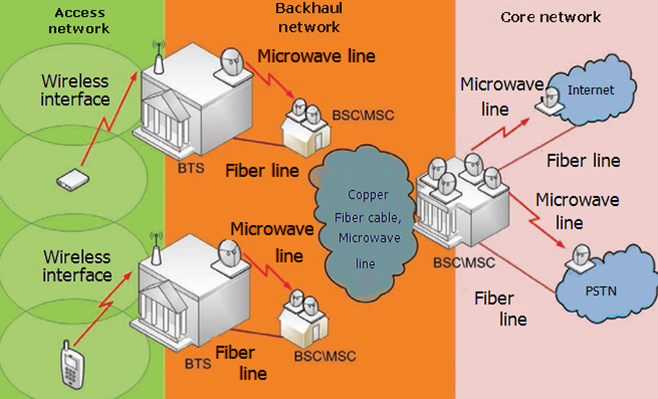
\includegraphics[scale = 0.35]{Pictures/network.png}

\caption{Real Architecture of Network} \label{network} 

\end{center}

\end{figure}



\section{NFD in NDN Networks}
NFD is a network forwarder that implements NDN forwarder. After the initial release, NFD became a core component of the NDN Platform and will follow the same release cycle. 

There are different modules on NFD for different stuffs like \textit{core} which produce different varities between different modules of NFD. \textit{Faces} implements the face concept in NDN. \textit{Tables} which contains some data structures like Content Store (CS) and tables like FIB and PIB for forwarding and pending information for NDN Data/Interest packets and \textit{Forwarding}, which interacts with forwarding strategies to choose and manage faces and \textit{RIB Management} which implements routing table information about routes and each prefix according to proper faces. this is not a seperate module from NFD Management. Basically we create some faces for each prefix by a given routing strategy which are proposed in this work and it will fill up FIB properly against these information by which you find proper routes.

For example figure \ref{nfd} shows 2 faceIDs which are created by our proposed routing strategies in RIB and FIB: $67344$, $67876$. As you see these faces have routes toward 'jordan' and 'luca' thanks to strategies of TreeOnProducer.   

As you can see also in this figure there are different Forwarding strategies for different namespaces. We also added an option on Lurch to change it on run time.



\begin{figure}[H]

\begin{center}

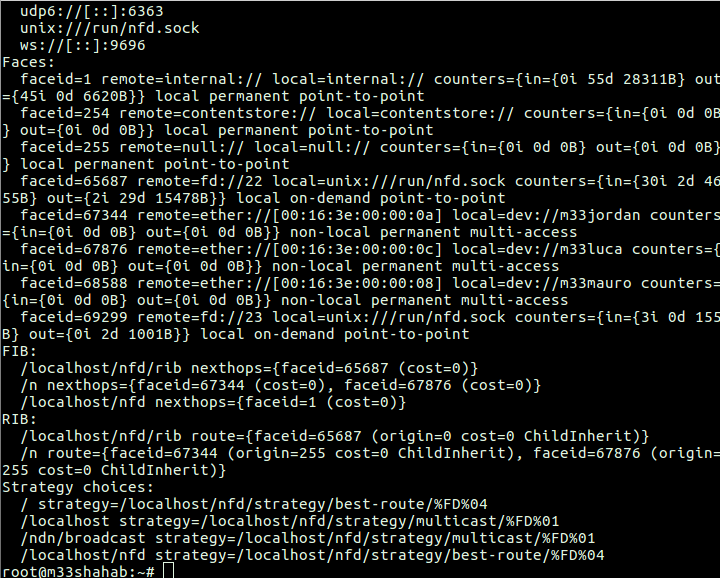
\includegraphics[scale = 0.35]{Pictures/nfd.png}

\caption{nfd-status on shahab container} \label{nfd} 

\end{center}

\end{figure}


Picture \ref{nfd} shows well that there is no route for 68588 in RIB which means as \cite{jacobson} also says forwarder engine needs a Software to do this kinds of selection which explains very well the reason why we work on these strategies. Each forwarder must decides this selection using proper strategy. 

%----------------------------------------------------------------------------------------
%	SECTION 1
%----------------------------------------------------------------------------------------
\section{Routing in NDN}
In NDN, the forwarding plane is the actual control plane
since the forwarding strategy module makes forwarding decisions on its own.  This fundamental change prompts us
to rethink the role of routing in NDN. Routing protocols are responsible for disseminating topology and policy information, computing routes and handling short-term network changes.

\textit{Shortest path}, \textit{Distance Vector}, \textit{Link state} and their variants IS-IS and OSPF are the routing algorithms that are most widely used inside large networks and the Internet of today from ARPANET (Bellman, 1957; and Ford and Fulkerson, 1962). (\cite{modulation})


 
\section{Routing Strategies}
\textit{ShortestPath} and \textit{Djikstra} algorithms are designed to obtain the paths which minimizes the cost metric of each link. 

In this subsection we introduce 4 different algorithms which are defined in function of network's need for NDN networks.

We will also mention the ideas and reseaons for these strategies. Next section we will show some results and figures about algorithms for one medium size and large size of network.

In this work we will work on Shortest path using different metrics. Basically number of hops for links in order to calculate our routes properly in function of network postion.

\textit{ShortestPath} In \textit{Networkx} Python library is called \textit{Unweighted} method for Graph becasue it assumes number $1$ for each link which is simply number of hops. In ndnSim which is an ndn simulator, this weight has been put $1$ because of NDN. In this library \textit{Djikstra} is called \textit{weighted} methods becasue it cares about the number of weight to which the link is mapped and it's the way how it obtains proper paths. 

For Discovering more about algorithms we refere you to \ref{Appendix} to see the details of implementation. 

\subsection{Consumer $\&$ Producer Trees Strategy}
In ICN the cost metric is \textit{number of hops} becasue of naturity of ICN architecture in which you \textit{search} content so basically in Graph sense nearer nodes are preferred always. This is the idea that enables us to think about \textit{TreeOnConsumer} and \textit{TreeOnProducer} strategies in which you want to find the tree which finds the shortest paths either from one producer to consumers or one consumer to producers properly.

The idea of \textit{TreeOnConsumer} is based on this concept that imagine once in cellular networks at the same time maybe you can have $N$ clients or consumers that search exactly the same \textit{content}, like a special video. Figure \ref{consumer} shows this concept properly.


\begin{figure}[H]

\begin{center}

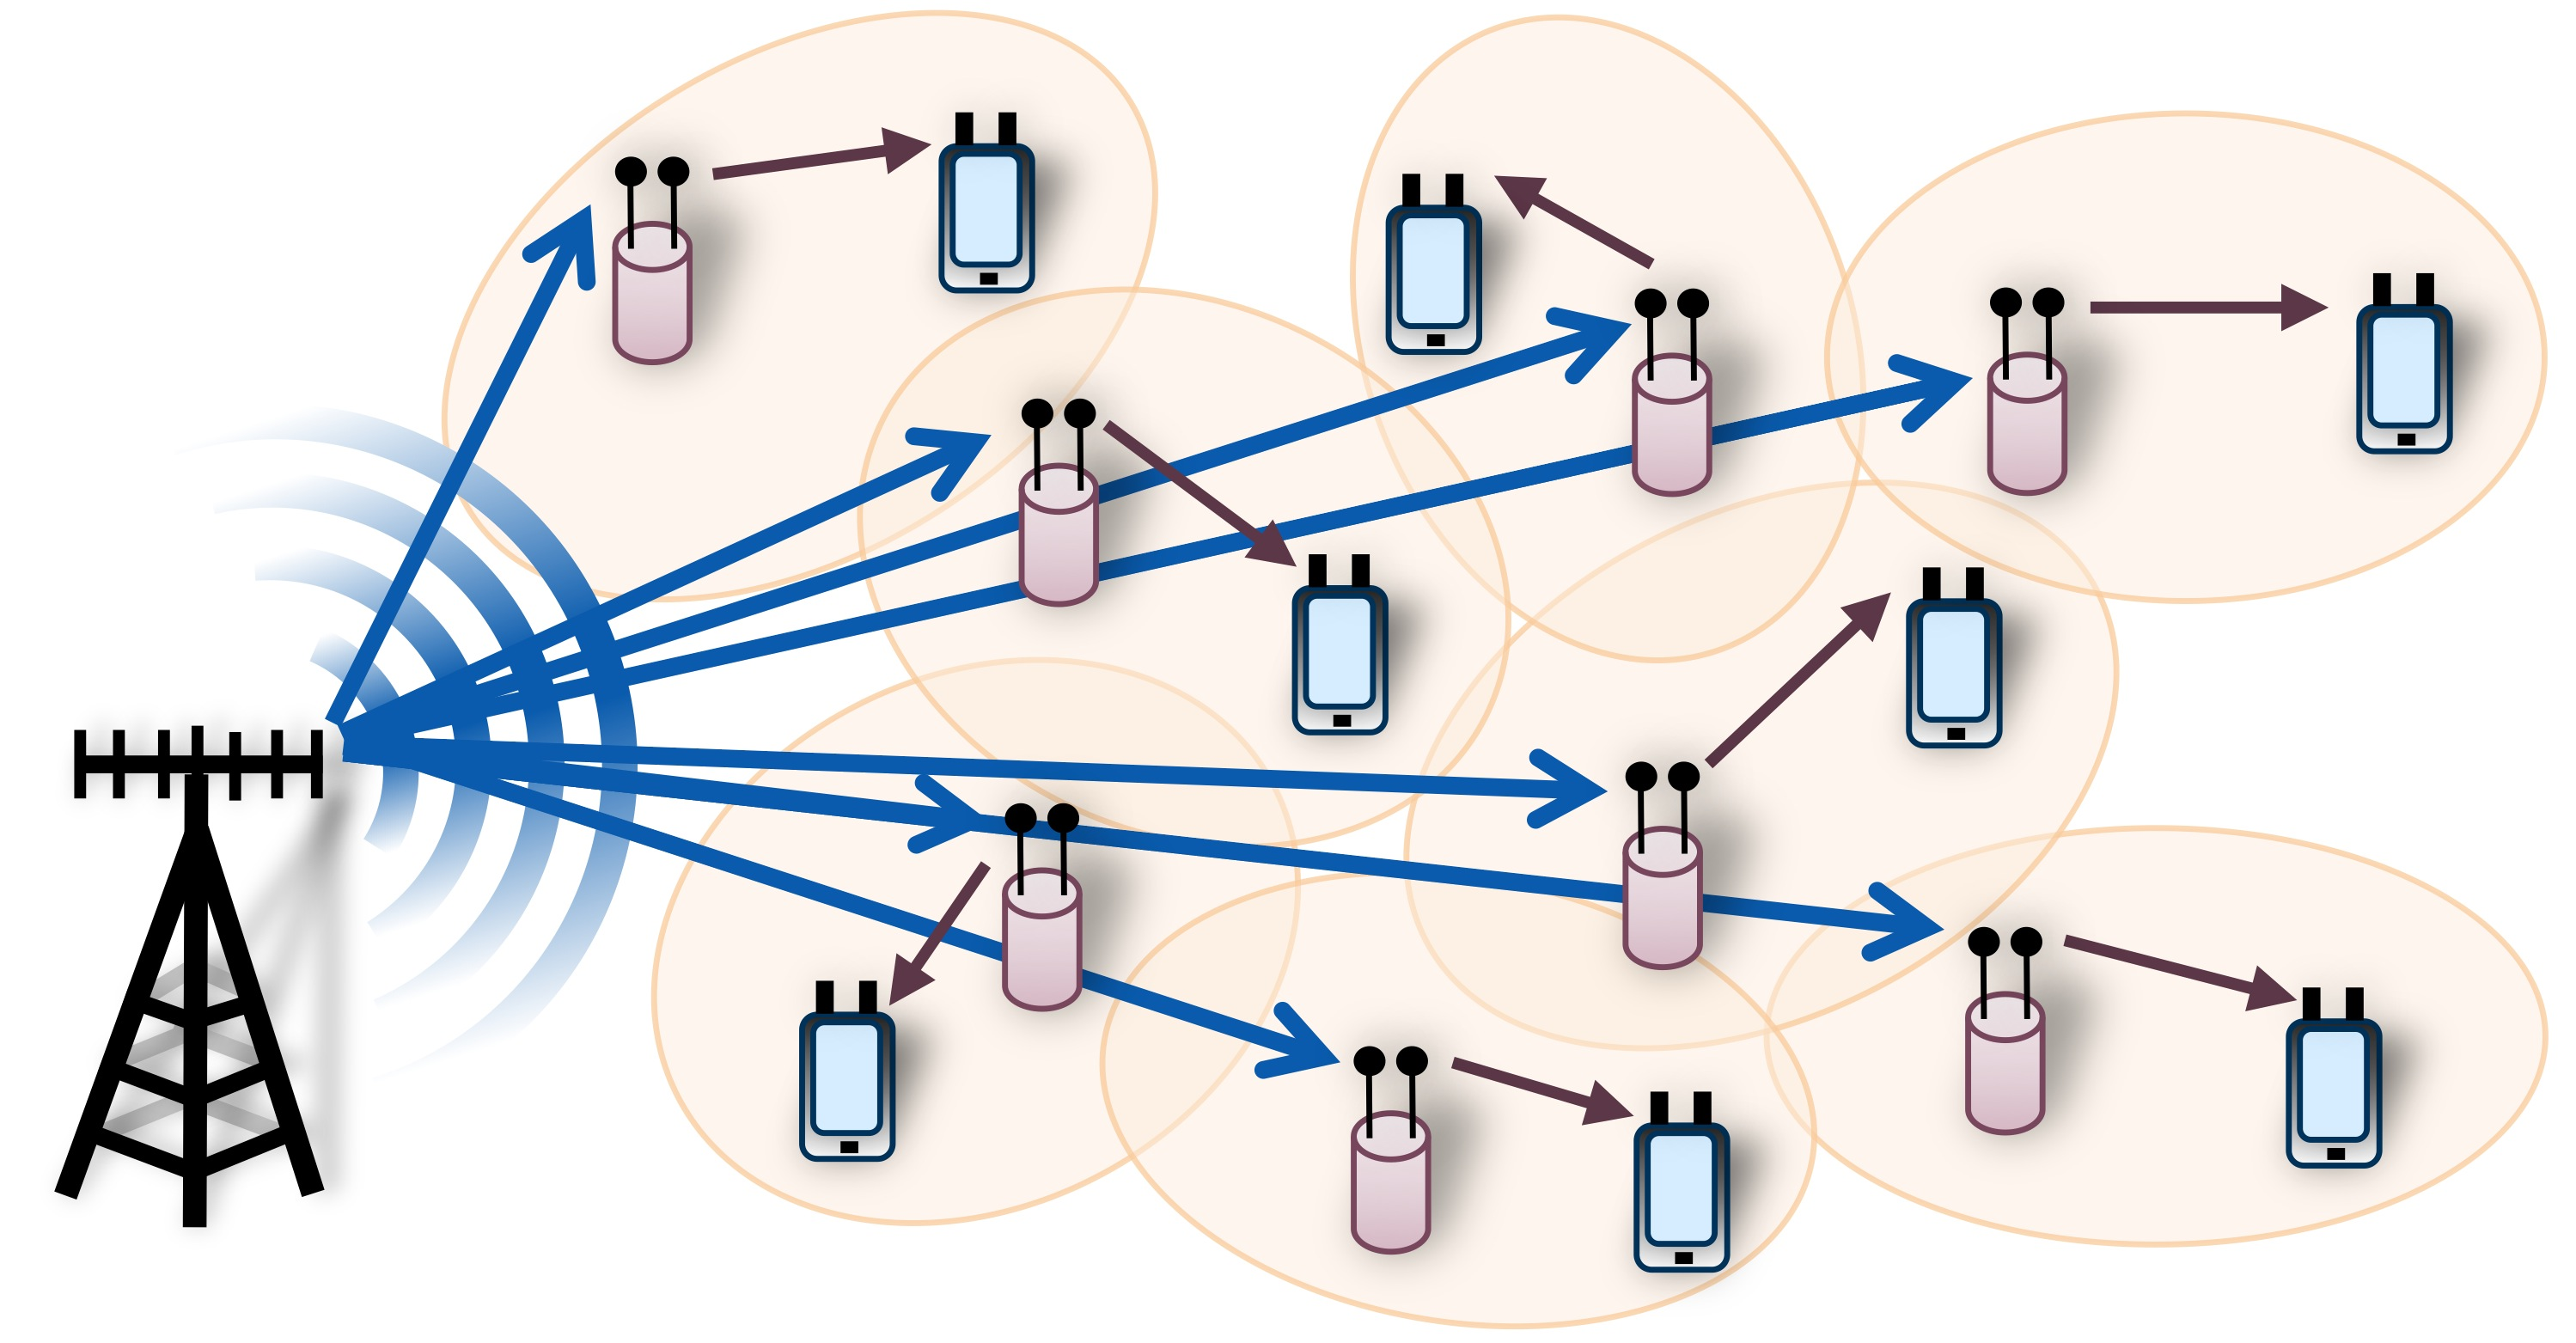
\includegraphics[scale = 0.1]{Pictures/treeonconsumer.jpg}

\caption{TreeOnConsumer} \label{consumer} 

\end{center}

\end{figure}
     

\textit{TreeOnProducer} is a bit inverse thinking of previous algorithm, in which imagine you, as a client to speed up your video downloading you can retrive your data using different repositories packets to catch up (Figure \ref{producer}).

\begin{figure}[H]

\begin{center}

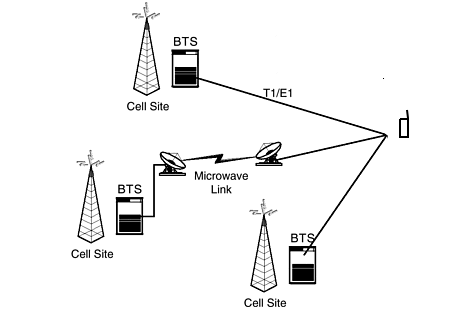
\includegraphics[scale = 0.4]{Pictures/treeonproducer.png}

\caption{TreeOnProducer} \label{producer} 

\end{center}

\end{figure}

So the idea of \textit{TreeOnProducer} is to use all of network available repositories on the core part of the network by this way imagine a case of very dense clients on one cell network will be able to understand the amount of demands and to respond them at the same time using this strategy to have maximum possible usage of network. 

\subsection{Minimum Cost MultiPath Strategy}
Imagine a case you have multiDestination, like a live videostreaming football match that has a lot of viewers in the network at the same time, in this case nodes should do some kind of multicast sending packets to the networks so network should choose the routes which minimizes the cost of links from source to destinations. The cost is always number of hops in ICN context because of naturity of architecture. 

Figure \ref{balance} shows well the idea of this strategy which is designed for multi-destination case with minimizing cost.

\begin{figure}[H]

\begin{center}

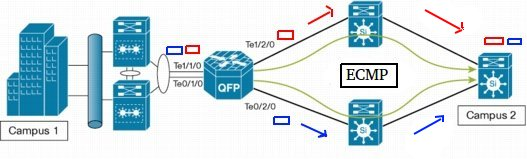
\includegraphics[scale = 0.7]{Pictures/balance.jpg}

\caption{Eqaul Cost Multipath Strategy on CISCO Router} \label{balance} 

\end{center}

\end{figure}

As you can see in \ref{balance} is a simple topology example of real cisco routers implemented between 2 campus in this case you can deliver packets, one by one wich means packets can travers through one upper path and the other with belower path.

\textbf{Multi-Producer, Multi-Consumer} is when you have multiple consumers who are searching the same content and multiple producers for this content. This algorithm is the core of the strategies becasue of its ability. Actually this algorithm looks at the position of clients and producers then for each client finds the closest producer (as we said number of hops is always our metric) then routing is done.



\subsection{Maximum Flow Strategy}
This strategy is done by calculation of paths and links which produce maximum throughput from source node to sink node. \textit{MaxFlow} is very important strategy which allows the links to participate in subgraph which maximizes the capacity and basically it creates an one-directed graph and all ratio traffic through these links should be calculated by this strategy. Figure \ref{max} shows well this explanation. Algorithm has chosen paths which maximizes flow to the sink node.

\begin{figure}[H]

\begin{center}

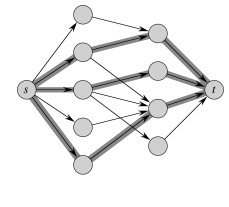
\includegraphics[scale = 0.8]{Pictures/max.jpg}

\caption{Maximum Flow Strategy} \label{max} 

\end{center}

\end{figure}


 
Specially this strategy can be used when mobile phones want download video packets with very high quality video coding rates (i.e Ultra HD ,4K, ...) or to speed up downloading content and the network allows to get information through different paths from sources to clients. This strategy works with a weight (\textit{capacity}) on each link.

As it's clear there is some paths which are not selected becasue it wouldn't produce total maximum flow on network.  The idea of this strategy is to use throughput capability of network to achieve to have the best quality at the edge user experience. 

This can be usefull whenever imagine a case the base station as a one cellular have to decide a lot of connected mobile stations at the same time. This needs a heavy packet transmission to all clients. Imagine also if all clients want to see a 4K video, so how much data should network be able to transfer to all clients. This decision can be taken by Lurch in which you are able to say to this base station to send the packets.

 





 
% Chapter Template

\chapter{Experimental Results on Routing Strategies} % Main chapter title

\label{expereince}

\lhead{Chapter 2. \emph{Experimental Results on Routing Strategies}}

\section{Experiment Test Setup}
We tested our experiments on clusters of cisco's server with linux containers with different configuration set ups on Lurch. In the case of needs, dynamic modifications also have been added on Lurch to be more interactive for different test scnearios.

In this chapter we will show, test and validate our 4 routing strategies on 2 different setup networks with 5 nodes (medium size) and another one with 17 nodes (large size) each one with costumized capacity. We plot rates in Kbps vs time for each link involved in strategy. $\{ai\}$, $i=$1:8 are Access Points and nodes with \textit{NodeID} are Autonomous nodes in the network.
   
In all scenarios we plot the figures of each link by nodeID of ends connected. In, Out means the direction of packets that come to node. We consider number of hops as cost of link as it is meaningful in ICN architecture.
\textit{TreeOnConsumer}, \textit{TreeOnProducer}, \textit{MinCostMultipath}, \textit{MaxFlow} are 4 different parameters of RoutingNDN module to choose which are done for \textit{Medium} and \textit{Large} size. We have put the result of each case inside the subsection.

In all cases Clients are searching /n/a/noseg chunk and repositories are containing /n folder which has alphabetical letters to like a,b,c,d, ... then chunks of \textit{BigBuckBunny.mp4} are appended to them. Engine of repository is an application called \textit{repo-ng}. 

\section{Strategies on Medium Size NDN Network}


\subsection{TreeOnConsumer}
As figure \ref{TreeOnConsumer} shows, 'luca' and 'jordan' nodes are clients searching '/n/a/noseg' chunk and 'shahab' node is producer of content. The first prefix of content is /n folder contains.

Figure \ref{treeonconsumer} shows 4 traced rates in which yellow and green one are data packets. Same packets are routed through \textit{TreeOnConsumer} tree to the clients with different rates. In this figure you can see the delay between 'sj' and 'sl' which is becasue of capacity difference of between containers. So you have 2 threads on 2 different machines occuring and recorded at the same time.

\begin{figure}[H]

\begin{center}

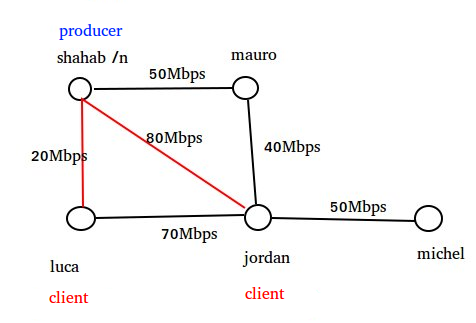
\includegraphics[scale = 0.4]{Figures/TreeOnConsumer.png}

\caption{TreeOnConsumer Tree Medium} \label{TreeOnConsumer} 


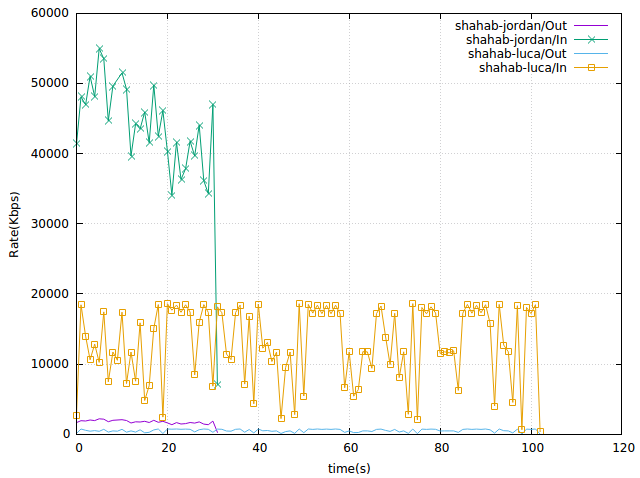
\includegraphics[scale = 0.4]{Figures/treeonconsumer.png}

\caption{TreeOnConsumer (Rate vs Time) Medium} \label{treeonconsumer} 


\end{center}

\end{figure}


\subsection{TreeOnProducer}
Figure \ref{TreeOnProducer} shows 'jordan', a client who searches '/n/a/noseg' and 2 producers ('shahab','mauro') who send packets to client by this strategy using tree of \textit{TreeOnProducer}. 
Figure \ref{treeonproducer} shows as well this downloading traced during time which can be used whenever client wants a high quality content.
\begin{figure}[H]

\begin{center}

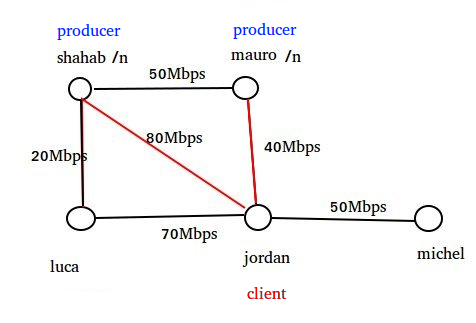
\includegraphics[scale = 0.4]{Figures/TreeOnProducer.png}

\caption{TreeOnProducer Tree Medium} \label{TreeOnProducer} 


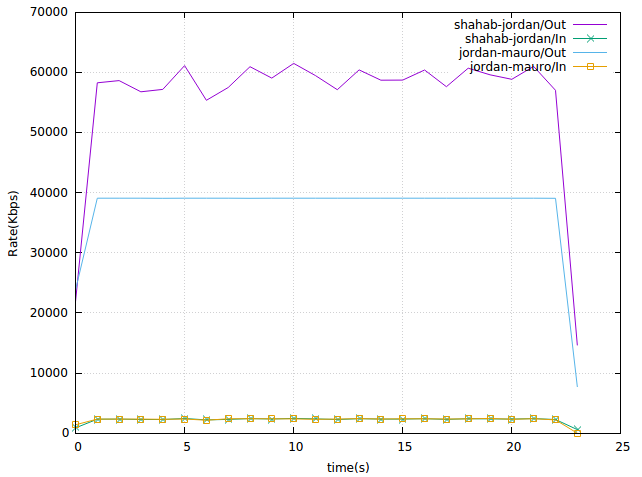
\includegraphics[scale = 0.4]{Figures/treeonproducer.png}

\caption{TreeOnProducer (Rate vs Time) Medium} \label{treeonproducer} 


\end{center}

\end{figure}

\subsection{MinCostMultipath}
Figure \ref{MinCostMultipath} shows \textit{MinCostMultipath} tree of minimum of network in which we use number of hops as cost of links. This is the case in which we want to broadcast video livestreaming as we discussed. Same chunk of datas are searching at the same time for a live movie like a football match content to all clients.
 
Figure \ref{mincost} shows traced data as well.
\begin{figure}[H]

\begin{center}

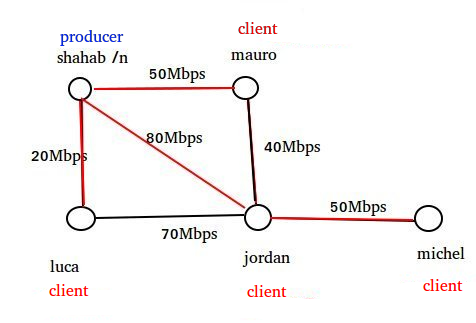
\includegraphics[scale = 0.4]{Figures/MinCostMultipath.png}

\caption{MinCostMultipath Tree Medium} \label{MinCostMultipath} 

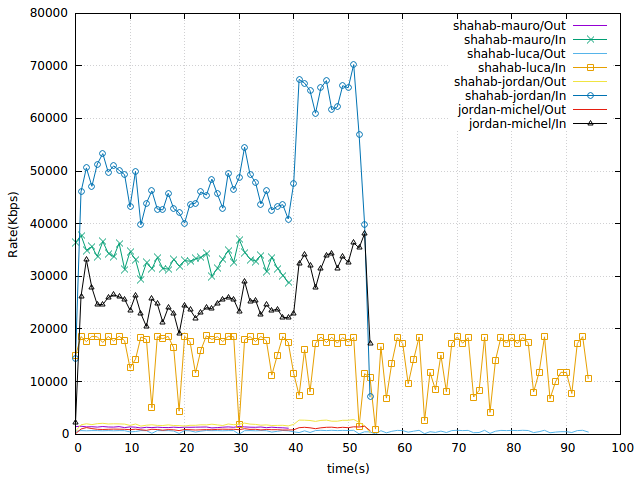
\includegraphics[scale = 0.4]{Figures/mincostmultipath.png}
\caption{MinCostMultipath (Rate vs Time) Medium} \label{mincost} 

\end{center}

\end{figure}

\subsection{MaxFlow}
In figure \ref{MaxFlow} 'jordan' node gets information from all of path possible to maximize data throughput.

Figure \ref{maxflow} shows data rates which are maximum for each link. It can be used whenever clients need higher quality data.

You can see for marginal paths you have on the stable rates.
\begin{figure}[H]

\begin{center}

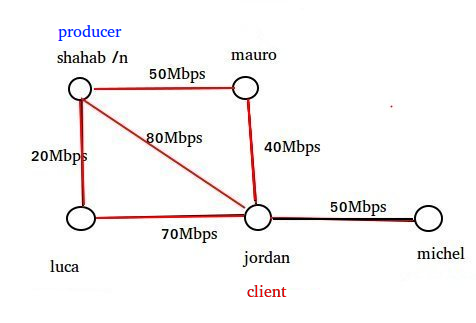
\includegraphics[scale = 0.4]{Figures/MaxFlow.png}

\caption{MaxFlow Medium} \label{MaxFlow} 


\end{center}

\end{figure}

\begin{figure}[H]

\begin{center}

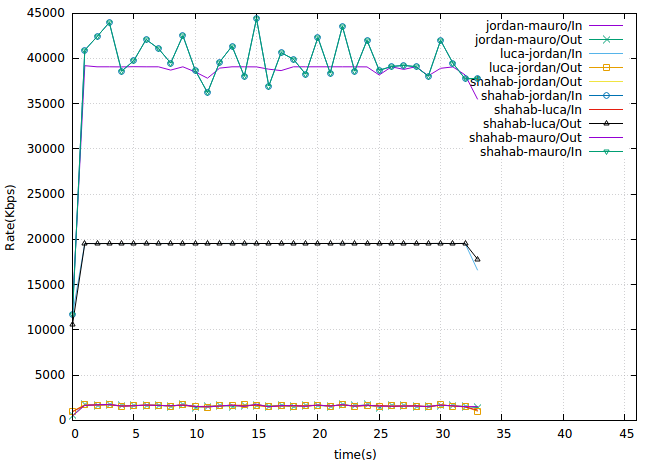
\includegraphics[scale = 0.4]{Figures/maxflow.png}

\caption{MaxFlow (Rate vs Time(s)) Medium} \label{maxflow} 


\end{center}

\end{figure}




 

\section{Strategies on Large Size NDN Network}

\subsection{TreeOnConsumer}
Figure \ref{TreeOnConsumer_big} shows a red subgraph, $a1, a2, a3, a4$ are Acces Points on which the mobile clients are connected through \textit{TreeOnConsumer} tree on the network.\\
In \ref{treeonconsumer_big}  rates are traced against time as well.

\begin{figure}[H]

\begin{center}

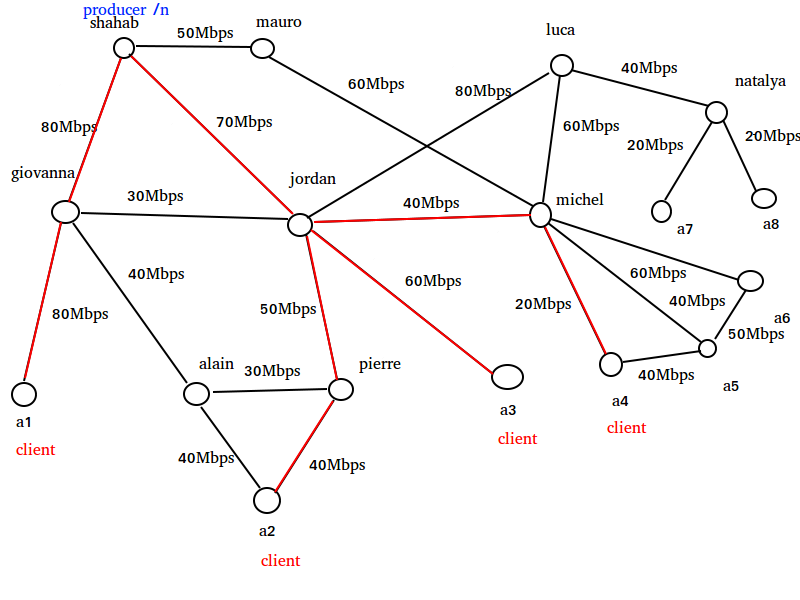
\includegraphics[scale = 0.4]{Figures/TreeOnConsumer_big.png}

\caption{TreeOnConsumer Tree Large} \label{TreeOnConsumer_big} 


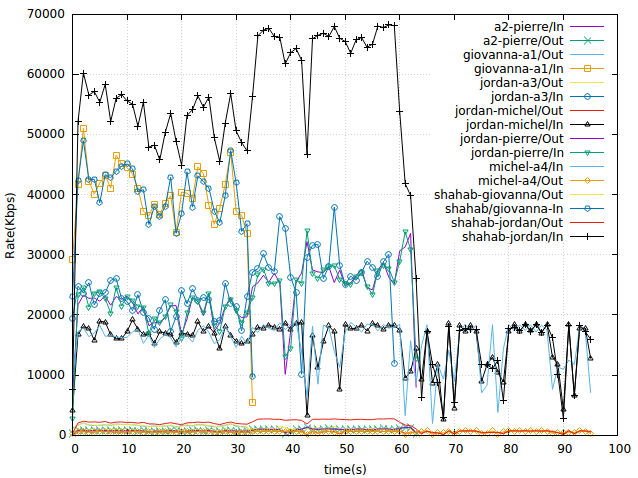
\includegraphics[scale = 0.4]{Figures/treeonconsumer_big.png}

\caption{TreeOnConsumer (Rate vs Time) Large} \label{treeonconsumer_big} 


\end{center}

\end{figure}


Figure \ref{Mob1} shows the first step of client mobility in which the mobile station is attached to node $n10$. Figure \ref{mob1} shows also the Interest/Data packets which are going through shortest paths.

You can see in figure \ref{Mob2} that as soon as mobile client is attached to $n11$ routing update is happened and new routing is traced.

Same case for \ref{Mob3} which is for showing that update can occured. This update can be designed periodically or to have an algorithm. After we need to know more practical constraints like how much time takes that an routing update happens? The answer depends on what we use for engine forwarder and its implementations. 



\begin{figure}[H]

\begin{center}

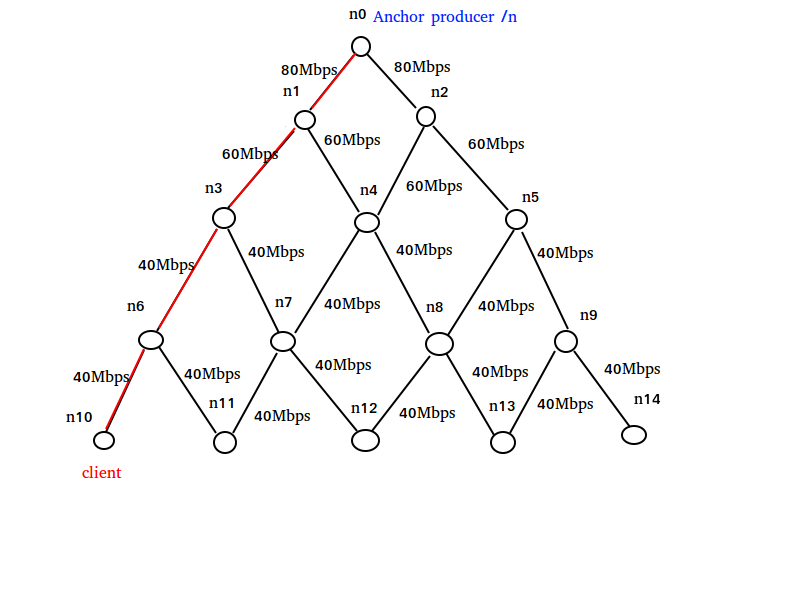
\includegraphics[scale = 0.4]{Figures/Mob1.png}

\caption{TreeOnConsumer Mobility Large} \label{Mob1} 


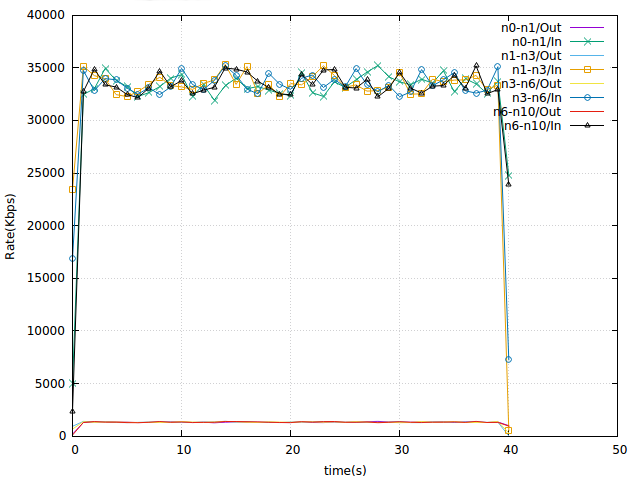
\includegraphics[scale = 0.4]{Figures/mob1.png}

\caption{TreeOnConsumer Mobility (Rate vs Time) Large} \label{mob1} 


\end{center}

\end{figure}

Now in figure \ref{Mob2} and \ref{Mob1} you see the rates which are changed whenever producer is changed. This changed is done mannually in this case.



\begin{figure}[H]

\begin{center}

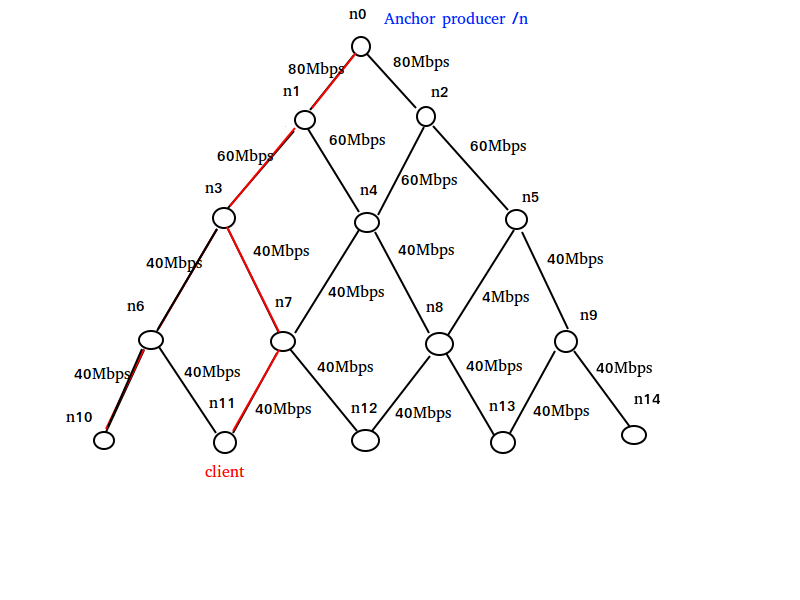
\includegraphics[scale = 0.4]{Figures/Mob2.png}

\caption{TreeOnConsumer Mobility Large} \label{Mob2} 


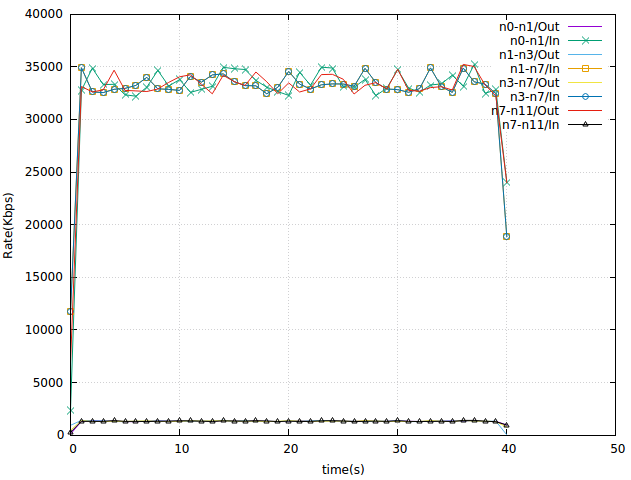
\includegraphics[scale = 0.4]{Figures/mob2.png}

\caption{TreeOnConsumer Mobility (Rate vs Time) Large} \label{mob2} 


\end{center}

\end{figure}

\begin{figure}[H]

\begin{center}

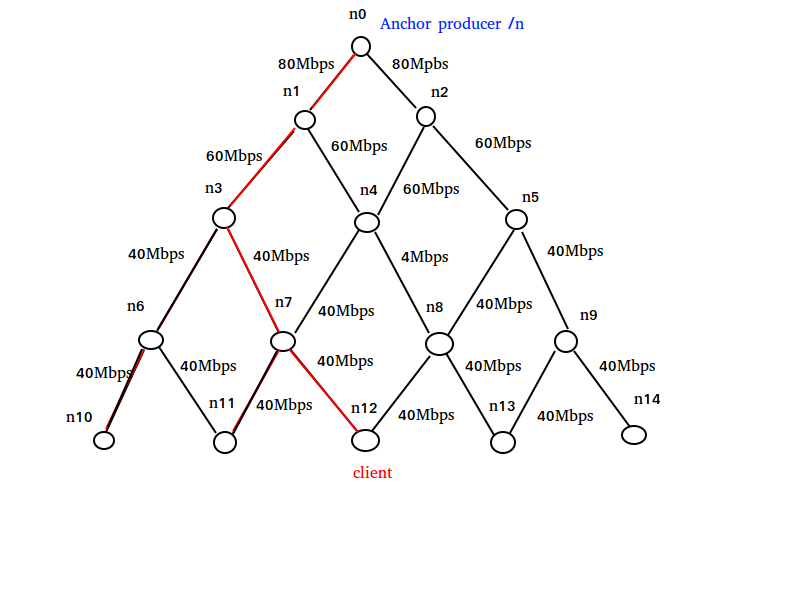
\includegraphics[scale = 0.4]{Figures/Mob3.png}

\caption{TreeOnConsumer Mobility Large} \label{Mob3} 


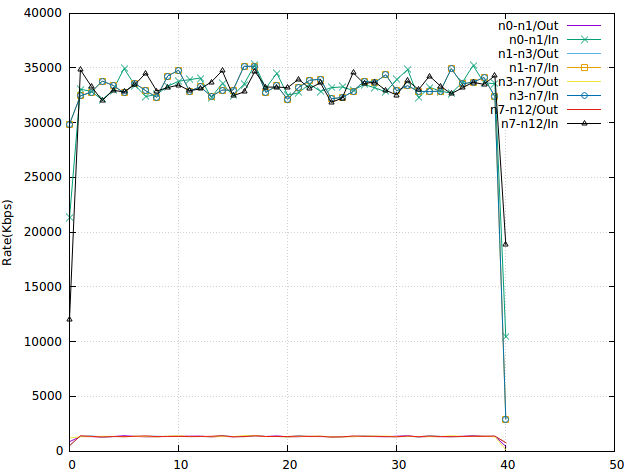
\includegraphics[scale = 0.4]{Figures/mob3.png}

\caption{TreeOnConsumer Mobility (Rate vs Time) Large} \label{mob3} 


\end{center}

\end{figure}





\subsection{TreeOnProducer}
Figure \ref{TreeOnProducer_big} shows $a6$ as Access Point client which recieves data from different producer nodes at the same time.

This strategy can be used whenever client can achieve to multiple repositories and it can download his chunk at the same time.

This is very usefull specially in case of load balancing strategy. Client can get his packets with different paths using different producers in the sense that maybe on the network mobile node wants download a higher data rates so he can use the benefit of multihoming of the content which is searching.

\begin{figure}[H]

\begin{center}

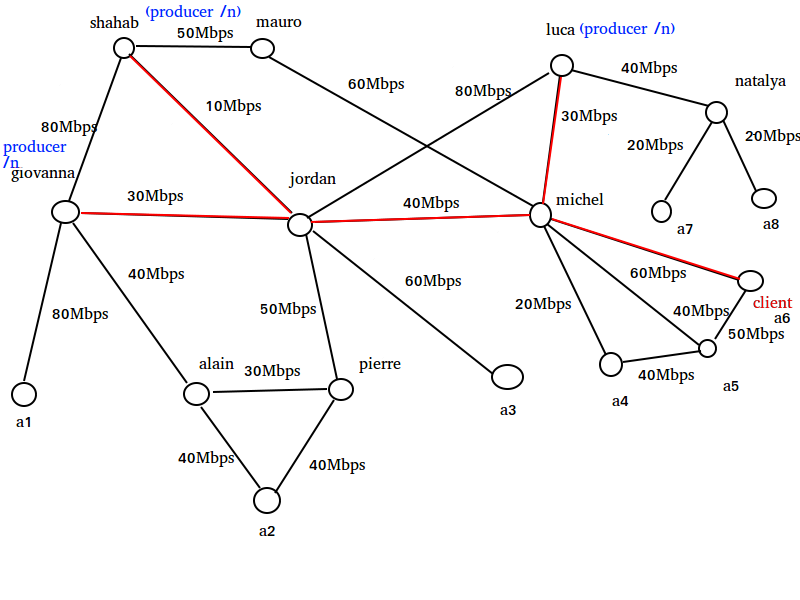
\includegraphics[scale = 0.4]{Figures/TreeOnProducer_big.png}

\caption{TreeOnProducer Tree Medium} \label{TreeOnProducer_big} 


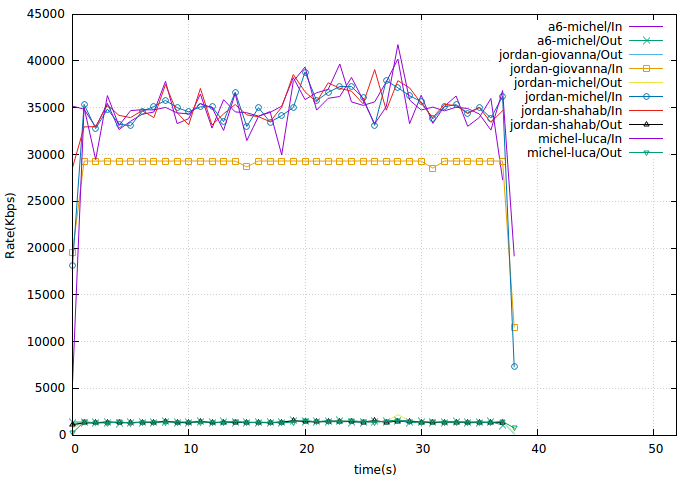
\includegraphics[scale = 0.4]{Figures/treeonproducer_big.png}

\caption{TreeOnProducer (Rate vs Time) Large} \label{treeonproducer_big} 


\end{center}

\end{figure}


\subsection{MinCostMultipath}
Figure \ref{MinCostMultiPath} shows how the \textit{MinCostmultiPath} tree is chosen to deliver content to all clients which are connected to access points.
 
Notably this strategy can be used when you want to do a \textit{Equal Cost Multi Path} (ECMP) routing in which your minimized paths have equal cost to destination so we should use load-balance or multipath forwading strategy to allow traffic to pass along the network. 

Figure \ref{load} shows well a simple case usage of this strategy using \textit{load balancing} strategy to use multipath routing.

\begin{figure}[H]

\begin{center}

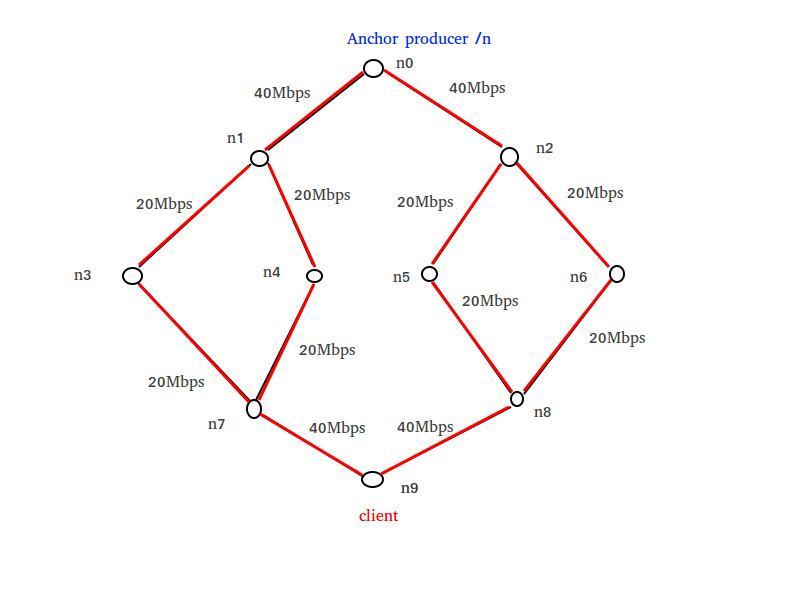
\includegraphics[scale = 0.4]{Figures/Load.png}

\caption{Multipath load balancing strategy Graph} \label{Load} 


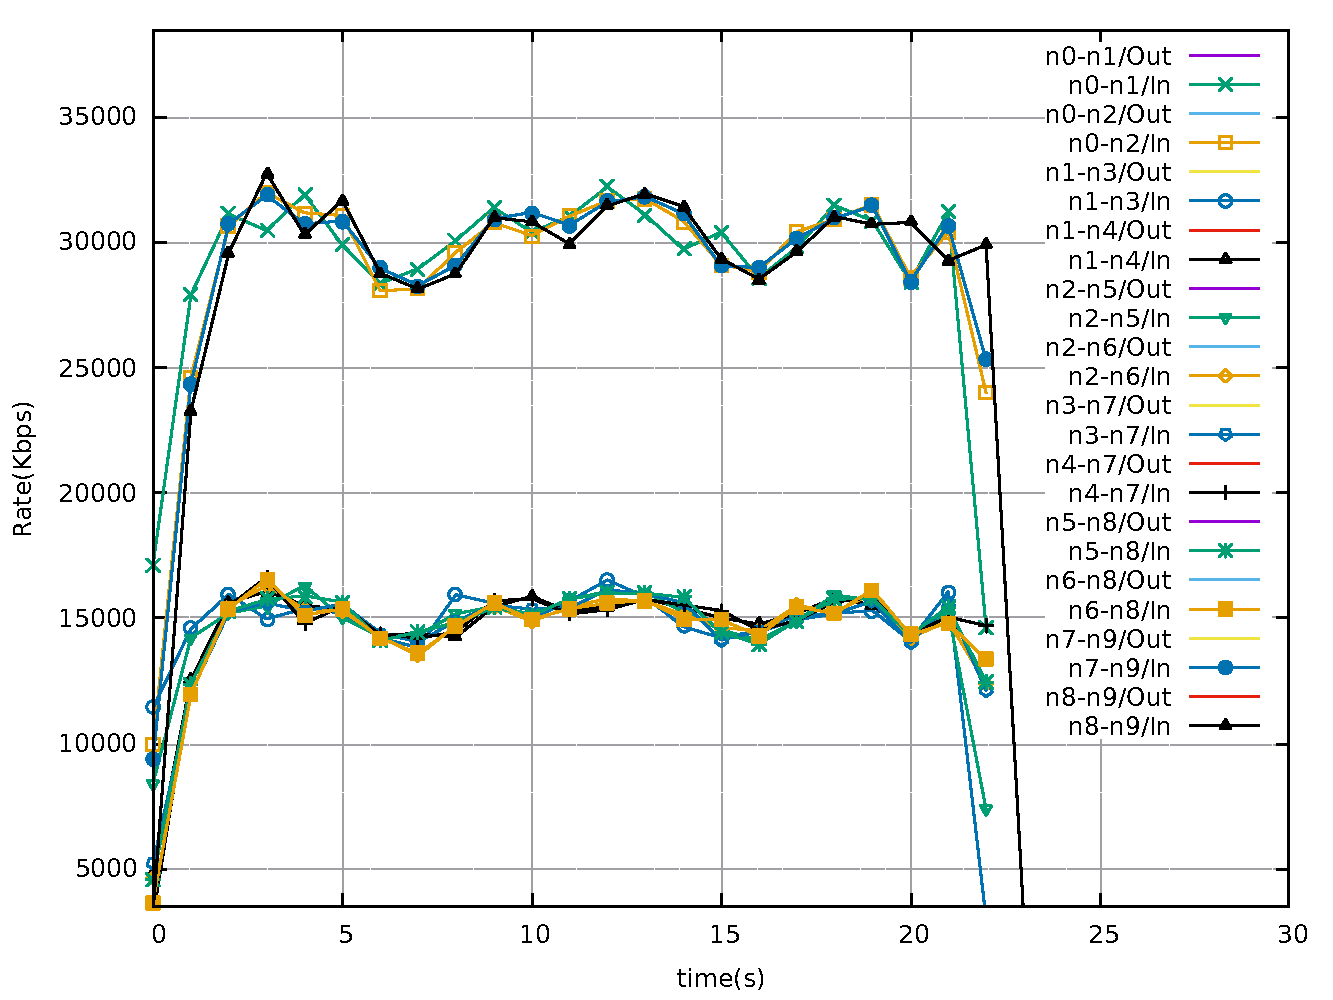
\includegraphics[scale = 0.4]{Figures/load.pdf}

\caption{Multipath load balancing strategy (Rate vs Time) } \label{load} 


\end{center}

\end{figure}




The algorithm of this strategy is written by the idea of searching minimum multipath from producer to client.

\begin{figure}[H]

\begin{center}

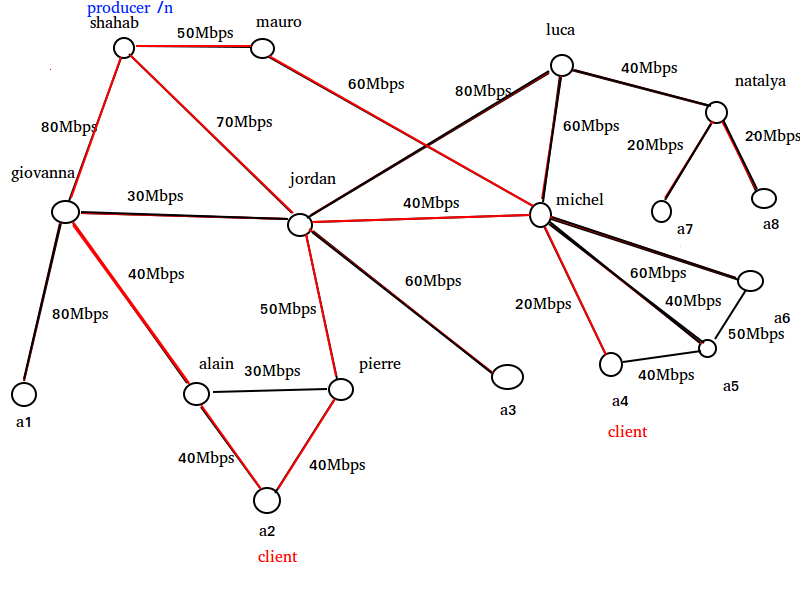
\includegraphics[scale = 0.4]{Figures/MinCostMultipath_big.png}

\caption{MinCostMultiPath Tree Large} \label{MinCostMultiPath} 


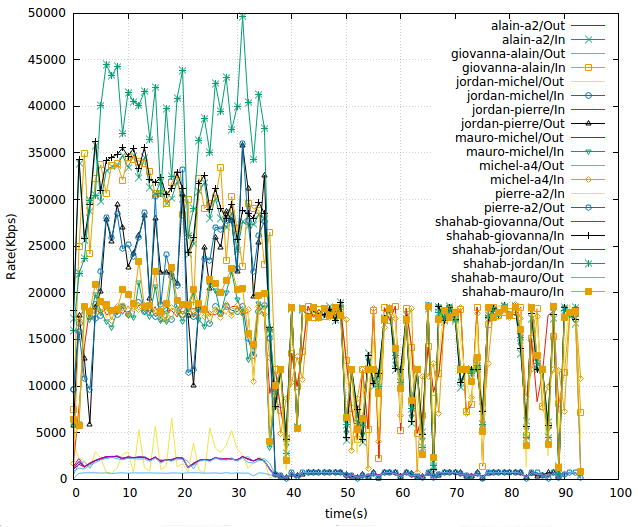
\includegraphics[scale = 0.4]{Figures/mincostmultipath_big.png}

\caption{MinCostMultiPath (Rate vs Time) Large} \label{mincostmultipath} 


\end{center}

\end{figure}


\textbf{\Large{Multi Consumers and Producers}}. Figure \ref{Multi-Repo-Client} as you can see we can have $n$ producers and $m$ consumers want to download at the same time. This strategy chooses the shortest paths between clients and consumers using to give routes update. Actually for each consumer, algorithm looks which producer is closer using \textit{shortest path} then set routes properly. This strategy can be very usefull in ICN networks becasue of its architecture. 

Routing is the core issues of any network even Network of streets and broadways! It's the idea of Routing in general is to have knowledge about network and its proper graph then have a table at each router to calculate best routes for each packet. This table can be static or dynamic, normally in practice routers are dynamic in function of network needs. 

One beautiful idea which is very \textit{à la mode} in research and development in these days becasue of its advantages is to have a \textbf{S}oftware \textbf{D}efine \textbf{N}etwork. The SDN can be a central controller who allows users to modify the network in terms of capacities, network topology, routing, and whatever you can think about the network which can be changes dynamically.

You can also imagine a scenario to occur, you can have algorithms inside algorithms to run full automate evidences. This strategy can be very usefull in these scnearios becasue of NDN architecutre.

By running this strategy on Lurch, it can understand whenever you want to do a ECMP or Multi repository client. It's important becasue network when you have your controller (Lurch) who understands the scenario in which you want to apply your strategies. 

  


\begin{figure}[H]

\begin{center}


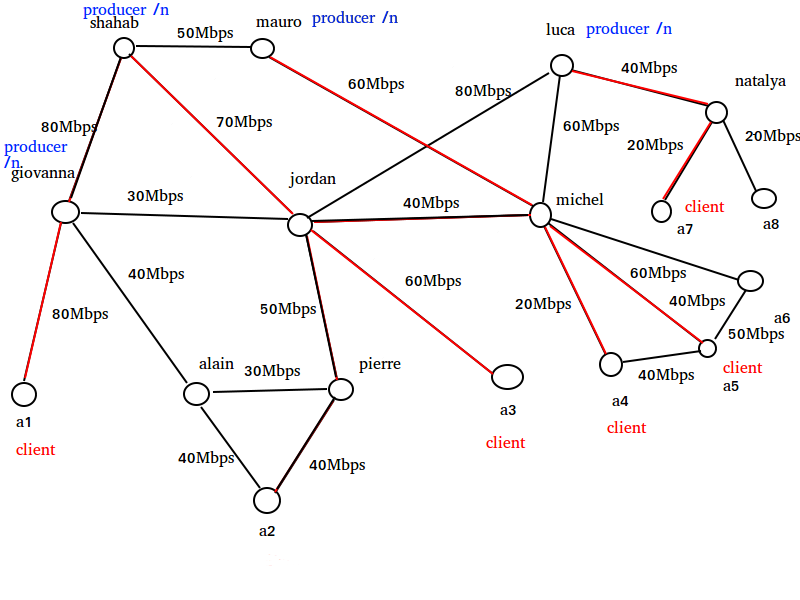
\includegraphics[scale = 0.4]{Figures/Multi-Repo-Client.png}

\caption{Multi Consumers and Producers Large} \label{Multi-Repo-Client} 


\end{center}

\end{figure}




\begin{figure}[H]

\begin{center}


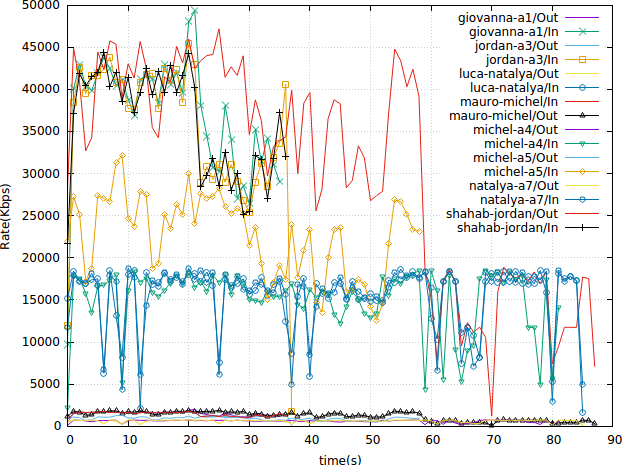
\includegraphics[scale = 0.4]{Figures/multi-repo-client.png}

\caption{Multi Consumers and Producers (Rate vs Time) Large} \label{multi-repo-client} 


\end{center}

\end{figure}

Now let's consider an interesting point of this strategy in Mobility of ICN. Figure \ref{Step1} shows the first step of a mobility scenario in which producer is attached to n18. In this case producer can be a Robot carrying a webcam to capture a film from environment send it to network as the content producer. The clients are mobile stations and are attached to base stations as well.   


\begin{figure}[H]

\begin{center}


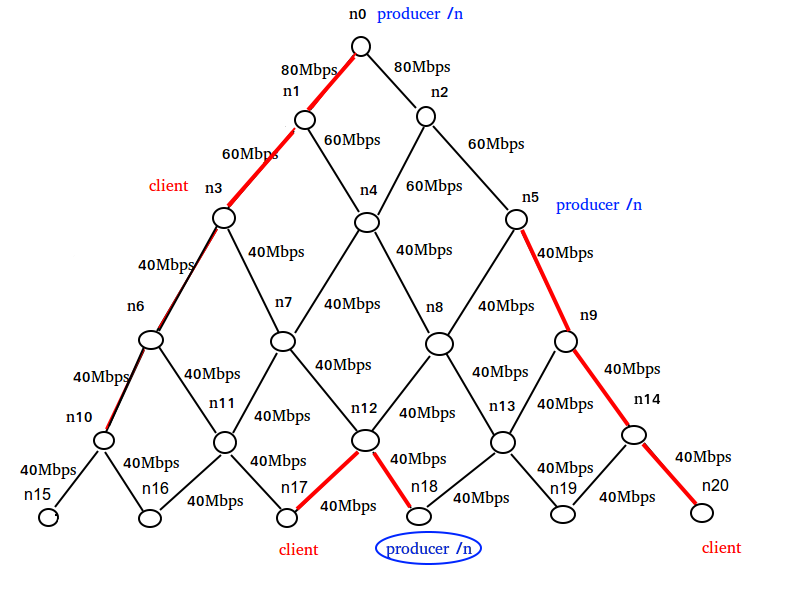
\includegraphics[scale = 0.4]{Figures/Step1.png}

\caption{Producer Mobility step 1} \label{Step1} 


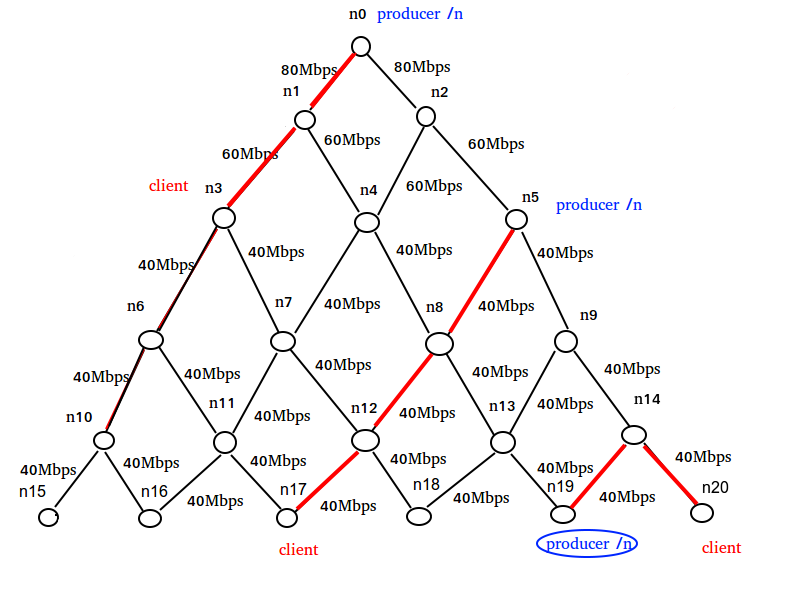
\includegraphics[scale = 0.4]{Figures/Step2.png}

\caption{Producer Mobility step 2} \label{Step2} 

\end{center}

\end{figure}






\begin{figure}[H]

\begin{center}

\includegraphics[scale = 0.4]{Figures/step1.png}

\caption{Producer Mobility step 1 (Rate vs Time) Large} \label{step1} 


\includegraphics[scale = 0.4]{Figures/step2.png}

\caption{Producer Mobility step 2 (Rate vs Time) Large} \label{step2} 


\end{center}

\end{figure}



Now let's consider a case which i call it \textit{Dense} network becasue the number of clients and repositories are more than rests.

Figure \ref{Dense} shows well automatic routing best shortest path for each consumer to achieve to producers using this strategy.

Figure \ref{dense} shows also the stairs of rates falling down in the network becasue of waterfall sense of Network. Basically more you go deeper to network the capacity rate will be increased which is real assumption in networks becasue (backbone / backhaul / Mobile edge, ...)
\begin{figure}[H]

\begin{center}


\includegraphics[scale = 0.4]{Figures/dense.png}

\caption{Dense Network} \label{Dense} 

\includegraphics[scale = 0.4]{Figures/dense.pdf}

\caption{Dense Network (Rate vs Time) Large} \label{dense} 


\end{center}

\end{figure}












\subsection{MaxFlow}
Figure \ref{MaxFlow_big} shows the paths chosen by strategy to maximize the throughput. This strategy works with capacity of each link and according to these value it returns the paths which can maximum the throughput toward clients.

Figure \ref{maxflow_big} shows how the rates are changing during time with this strategy. As you can see data packets have maximum value to achieve the output.  

The mobile stations are connected to $a2,a3$ Access Point can download their contents through taps interfaces.

The algorithm of this strategy is written by finding the paths which maximize throughput with preventing out of range extra loops.

\begin{figure}[H]

\begin{center}

\includegraphics[scale = 0.4]{Figures/MaxFlow_big.png}

\caption{MaxFlow Tree Large} \label{MaxFlow_big} 


\includegraphics[scale = 0.4]{Figures/maxflow_big.png}

\caption{MaxFlow (Rate vs Time) Large} \label{maxflow_big} 


\end{center}

\end{figure}




%% Chapter Template

\chapter{Experiments on New Routing algorithms} % Main chapter title

\label{coding}

\lhead{Chapter 2. \emph{New Channel Codings}}

\section{Objectives and Scopes}
In this Chapter we are interested in developing system with adding blocks called \textit{Channel Coding}, it's clear that it must add it before all of signalling blocks of Figure \ref{system3} because the idea of channel coding is just adding some logically redundancy bits to permit to receiver at first to detect errors and then the ability of correction in packets. DASH7 protocol uses a channel codings and our scope is to propose a new channel codings to enhance the performance in terms of bit error rate of system.

In information theory, the noisy-channel coding theorem (Shannon's theorem), establishes for any given degree of noise contamination of a communication channel that it is possible to communicate digital information nearly error-free up to a computable theoretical maximum rate which can be calculated by \ref{shannon} through the channel. The Shannon limit or Shannon \textit{Capacity} of a communications channel is the theoretical maximum information transfer rate of the channel, for a particular noise level (SNR). In equation \ref{shannon} $B$ is the Bandwidth, $C$ channel Capacity and $SNR$ is the Signal to Noise Ratio power. Some people also are interested in $\frac{C}{B}$ which is called Spectral Efficiency (SE) of system. Each time that you appliy an Error Control Coding you will have a smaller SE which causes a smaller Bit Error Rate.  


\begin{equation} \label{shannon}
C = B \times log_{2}(1+SNR)
\end{equation}

Globally In Engineering One of the most important issues and parameters is the time that you want to put for a project or work, actually you can not never separate it from one of your minded parameters, it's the reason which for that in practice we are interested in Power and not just Energy, actually the power means the average energy that you can give to a project over time as job is very important, nor you can say easily i will stay 200 years to do my own project, while the technology is growing exponentially each day. So in this part heavily of calculation in function of processes done in code is very important also, more code is efficient more we have a short time to process calculation, for example in some  simulations we had to wait 3 days to obtain the exact results which I put it to do during the weekends to use more efficient of time. while we were using a 4-core dell processor.  
\section{Payload Packet Coding}
In DASH7 protocol has been previewed as we noted in Table \ref{frame_table} we have 2 parts to code, one is \textit{Payload + CRC} in which Payload comes from upper layers, after encapsulation by data link layer 'CRC' will be added at the end of this packet the second is \textit{header} which contains some information about given payload packet and it's ready to give this frame to physical layer to add syncornization part. In this subsection we will talk about coding of payload and the other will be applied on all this packet (without Syncronization) is Convolutional Channel Codes, in this subsection we will propose a new code \textit{LDPC (Low Density Parity Check)} which are named \textit{Capacity-Approaching Codes} because of their Bit Error Rates curves which are very near to Shannon limit against Convolutional codes and after that we will explain the different used algorithms.     

In first part we introduce the curves of BER and BLER for different Coding in different channel, the next part is to introduce the \textit{LDPC} \& \textit{Convolutional} channel codes and then we explain mathematical equations and ideas of Encoding and Decoding algorithms.
  

\subsection{BLER and BER Curves in Different Channel Models of Different Codings}
The BER vs SNR is the curve of Bit Error Rate against of signal to noise ratio, in digital modulation is 
$\frac{E_{b}}{N0}$ which definitely depends on Modulation and Signal Shaping. it's defined by the number of received error bits in packets, divided by the length of packet with an acceptable statistical of test. It means for watching bit error rate of $10^{-4}$, it should have at least $10^{4}$, actually theoricaly it's correct but in practice for a good immunity for example this error probability we test $10^{5}$ or $4 \times 10^{4}$.
BLER is just a measurements which is used more in higher layers (data link, ...) which means that the number of received errors packet.

Figure \ref{ber} is the bit error rate of coherent demodulation without coding of DASH7 (2-FSK, with index of modulation of 1.8 \& 0.5) which by increasing when $h = 0.5$ is better because the discontinuity of signalling is lesser in this case. We can say that BLER is proper to BER, so from this time we only concentrate on BLER curves, because it is more important in terms of protocols.    

Now figure \ref{bler_coding} shows Block Error Rate of system \ref{system3}, clearly the difference between system with coding convolutional and without coding. You can see also a better curve (green) which is better when we put \textit{Zero Padding}. Actually when we put a known word in the end of coding packet to help the algorithm State Machine steps for Viterbi (Hard Decoding). 

Figures \ref{bler_conv} and \ref{LDPC_Conv_final} are the competitions between LDPC and Convolutional coding, Figure \ref{LDPC_Conv_final} shows BLERs figures where LDPC starts to catch Convolutional codes which for \textit{Soft} decoding is about 4.2 dB and for \textit{Hard} decoding is about 5.2. Hard and Soft decoding for LDPC means 'Bit flipping' \& 'Log-Sum Product' and for Convolutional means 'Hard','Soft' decision of Viterbi algorithm. Details of algorithms will be discuessed in future subsection. In all figures packet bits test was for 16 Bytes (128 bits).   

In figure \ref{bler_conv} you can see there are 2 models of channel AWGN which is famous case of just added randomly noise to the transmitted signal and the second is TU5 which is a model of channel used in GSM system for 'Typical Urban' and is implemented by Jakes algorithms in Octave and figure \ref{LDPC_Conv_final} is in TU5 model channel \cite{urban}.

\begin{figure}[h]
\centering
\includegraphics[scale=0.8]{Figures/ber.jpg}
\caption{Bit Error Rate, 2-FSK modulation theory and simulation}
\label{ber}
\end{figure}


\begin{figure}[h]
\centering
\includegraphics[scale=0.9]{Figures/bler_coding.jpg}
\caption{BLER, with \& without Coding, Zero Padding}
\label{bler_coding}
\end{figure}


\begin{figure}[h]
\centering
\includegraphics[scale=0.6]{Figures/bler_conv.jpg}
\caption{LDPC(256,128) and Convolutional in AWGN \& TU5 channel model}
\label{bler_conv}
\end{figure}

\begin{figure}[h]
\centering
\includegraphics[scale=0.6]{Figures/LDPC_Conv_final.jpg}
\caption{BLER of LDPC(256,128) vs Convolutional Coding with Hard and Soft decoding}
\label{LDPC_Conv_final}
\end{figure}
   
\subsection{LDPC and Convolutional Codes}
In this subsection we are going to explain problems with theoretical and mathematical description.
Globally Error Control Codes are divided by 2 parts 'Convolutional' and 'Block Linear' codes.

Now we are interested in presenting our new channel coding, \textbf{LDPC} codes, which are very high performance and have strong results in Bit Error Rate curves.

Historically, these codes first developed by Gallager in 1963, and then were forgotten until his work was rediscovered in 1996, Turbo codes, another important class of capacity-approaching codes discovered in 1993, became the coding scheme of choice in the late 1990s, used for applications such as the Deep Space Network and satellite communications, but in the last few years, the advances in Low-Density Parity-Check codes have seen them surpass turbo codes in terms of error floor and performance in the higher code rate range, leaving turbo codes better suited for the lower code rates only. 

In 2003, an irregular LDPC code beats six turbo codes to become the error correcting code in the new DVB-S2 standard for the satellite transmission of digital television. The DVB-S2 selection committee made decoder complexity estimates for the Turbo Code proposals using a much less efficient serial decoder architecture rather than a parallel decoder architecture. This forced the Turbo Code proposals to use frame sizes on the order of one half the frame size of the LDPC proposals.

In 2008, LDPC beat convolutional turbo codes as the forward error correction (FEC) system for the ITU-T standard.
G.hn chose LDPC codes instead of turbo codes because of their lower decoding complexity because the proposed turbo codes exhibited a significant error floor at the desired range of operation. LDPC codes are also used for 10GBase-T Ethernet, which sends data at 10 Gigabits per second over twisted-pair cables. In 2009, LDPC codes are also part of the Wi-Fi, 802.11 standard as an optional part of 802.11n and 802.11ac, in the High Throughput PHY specification.
These interests ,volunteers and reasons in LDPC codes caused to think about these codes for DASH7.

The main idea of \textit{LDPC (Low Density Parity Check)} is to produce a parity check matrix which are typically Low Density, means that the number of '1's bit are very smaller than '0's (0.001). It's the reason that codes are very practical for registering datas we need only to register '1's. there are many methods to construct LDPC codes such Gallagar, Prototype, Mackay Neal, Finite Geometry, RS based, Irregular, Random, ... .

In this internship we have tested the easiest to implement (gallagar, Regular, Mackay  Neal) because of practical objectives of internship and we chose Mackay Neal because of Figure \ref{ber_ldpc} which has gotten from \ref{Bibliography}, which is Bit Error Rate of 4 different codes, \textit{Rate 1/2 64 state convolutional}, \textit{Computer generated}, \textit{Mackay Neal} and \textit{EG-Gallagar} which can be concluded the best compromise between these codes, EG-Gallagar and Mackay Neal codes are the best performance in BPSK modulation in AWGN channel. Implementation of EG-Gallagar is difficult in practice. In contrast Mackay Neal codes are near to these codes and are more practical. So we chose Mackay Neal method to construct Parity Check matrix. LDPC codes are introduced using a sparse \textit{bipartite} Graph specially in Designing and Decoding Techniques\citep{errorcontrolcoding}.
    

\begin{figure}[h]
\centering
\includegraphics[scale=0.6]{Figures/ber_ldpc.jpg}
\caption{Rate-1/2 64 state Convolutional code, EG-Gallagar (512,256), Mackay Neal (504,252), Computer generated (512,252)}
\label{ber_ldpc}
\end{figure}



\textbf{Convolutional} codes are produced by shift registers which is actually a finite state machine and in function of states and input the output (binary coded) will be produced and  it's very useful and common in practice. Convolutional code used in DASH7 has a rate of 1/2, 3 shift registers with $G(D) = [\frac{D^3+D+1}{D^3+D^2+D+1},\ 1]$ matrix of generator which each $D$ is just an agent of a shift register and 1 is just moment input bit, 2 arguments is because of rate which means that it transforms each bit to 2 bit. Mathematical description let's say if you want to code a given bit for first output of Coding it's just enough to add (in $GF(2)$) all of the register's bits and the input bit and for second output is just enough to add the 3th, second and own bit input to have the 2 bits coded of your suitable bit.  

\textbf{Linear Block Codes}. The  general idea of these codes is to create a linear function (matrix) of binary bits which are basically produced by algebric structure and algebra abstract concepts which own-self obtained by algebric polynomials. These codes have 2 matrix, \textit{Generator}($G$), \textit{Parity Check}($H$) matrices. Generator matrix is a $k \times n$ matrix which $k$ is the number of message bits and $n$ is the length of coded binary stream just a matrix that you can multiply your binary stream and the results is the coded binary stream. There are different methods for Decoding of 'Block linear codes' one can be syndrome decoding algorithm. Actually Parity Check matrix  ($ (n-k) \times n$)permits us to understand if a binary stream is in codeword dictionary. We can check it by this method: Multiplying received bit stream by Parity Check matrix the result is called syndrome of stream. Syndrome is going to check, zero if there is no error in stream and if not by checking this stream in look-up table we can find the proper errors. In which look-up table is the correctable errors.



\subsubsection{Algorithms of Encoding}
\textbf{Algorithm of Encoding of convolutional} coding is by a 3 state memory shift register. The circuit is shown in Figure \ref{conv_block} which just transforms each bit to 2 bits depends on last moment state and input now, equations of matrix generator produce the coded message $G(D)$ form a feedback in practice to be stable so they are usually normalized.

\begin{figure}[h]
\begin{center}
\includegraphics[scale=0.4]{Figures/encoder.png}
\end{center}
\caption{Logical Circuit of DASH7 Convolutional code}
\label{conv_block}
\end{figure}


Actually as we said encoding of linear blocks codes are done by a matrix generator called ($G$) which is just simply a multiplication, the other hand, basically constructing LDPC codes are done by Parity Check Matrix ($H$, which are low density), the problem is for encoding it must transform $H$ to $G$, actually this procedure is not easy, specially when dimensions of parity check matrix is large. In my internship because we wanted to code payload and the minimum acceptable of payload was 16 Byte, we have chosen a parity matrix of 128$\times$256, which means that the rate of coding is $\frac{1}{2}$ and is constructed by \textit{Mackay Neal} method and we have 128 redundant bit for 128 bit message.          

\textbf{Method of Mackay Neal LDPC} is based on producing random columns of $H$ matrix such that there will find no 2 columns or rows as vectors that have maximum in one place the same '1' common. This is because of preventing 4-cycles girth in proper graph The steps of algorithm is this: 1) Producing all zero matrix $M \times N$, 2) In all columns of H and some of rows there will be $\gamma$ bit '1' 3) Become randomly the rows that consists any or just one bit of '1' to 2 bit '1'. 4) In each , $\rho = \frac{N_{\gamma}}{M}$ , must be an integer number if $\rho$ is not an integer, it can not be designed a regular code. 5) If the weight of $ith$ row is greater than $\rho$ randomly  one of the bit '1' of this row is chose and it exchanges with another rows which have a smaller weight against $\rho$, if there is no row by this condition it repeats for the columns. 6) Preventing the 4-cycle path in proper graph.     

There are also another methods which are just the subsection of this algorithm, which can be generated by producing 2 submatrices seperatley cunstructed by LDPC methods.

\textbf{Girth of LDPC}. In LDPC Parity Check matrices there is a parameter called \textit{girth} of matrix, is just a parameter in LDPC codes which demonstrate the degree of ability of code some increasing in girth which progress the performance is basically to prevent 4-cycle in Tanner graph of code. One of the most important challenges in LDPC codes is \textit{Cycle Decomposition}, 4-cycle (vertices of rectangle of bit '1') in $H$ it can be heavily degraded the performance of code.  Bipartite graph of code searches all of equations to be satisfied to be correct or not. Actually for preventing of these 4-cycles we transform each columns or rows of $H$ by 2. This procedure is called \textit{Cycle Decomposition} and we'll have an expanded code in which the cycle of parities check is lesser and it can increase the performance of code. This algorithm prevents these 4-cycles. We have used an \textit{irregular matrix code with $\rho = 3$ \& $\gamma = 6$ are the mean of rows, column's Hamming weight}. In practice Irregular LDPC codes are more useful because of their better performance.

\textbf{Encoding LDPC}. Compared with general linear block codes, LDPC encoding with \textit{Lower Triangular Check Matrix} and \textit{Approximate Lower Triangular Check Matrix} carry out encoding directly by parity check matrix $H$. There are two types of encoding by lower triangular check matrix structure. The first is to use the Gaussian elimination to convert the check matrix H into lower triangular matrix structure before encoding. The encoding complexity is $O(n^{2} )$, $n$ is the column of check matrix. However, lower triangular check matrix produced in this method is not consistent with the sparse characteristics. The second is to directly use a given lower triangular sparse check matrix for encoding, which may result in loss of encoding performance.

Approximate lower triangular LDPC encoding was proposed by Richardson and Urbanke in 2001. The encoding is to disintegrate the check matrix H (as shown in Figure \ref{matrix}) into six ($A, B, C, D, T , E$) sparse sub-matrix before working out the redundant bit $p1$ , $p2$ (Equations \ref{matrixeq}) according to the characteristics of the six sparse sub-matrix to complete the encoding. The encoding complexity is $O(n + g^{2})$, $g$ is the row of matrix $E$. Compared with the lower triangular encoding matrix, the complexity is lower and the encoding is consistent with the sparse characteristics; hence, the encoding performance is relatively higher. Coded message will be $c = [m, p1 ,p2]$.
\begin{figure}[h]
\centering
\includegraphics[scale=0.6]{Figures/matrix.jpg}
\caption{Left : Lower Triangular Check Matrix , Right : Approximate Lower Triangular Check Matrix }
\label{matrix}
\end{figure}


 
\begin{equation} \label{matrixeq}
\left\{\begin{matrix}
Am + Bp_{1} + Tp_{2} = 0 \\
(-ET^{-1}A + C)m + (-ET^{-1}B + D)p_{1} = 0
\end{matrix}\right.
\end{equation}

\begin{equation}
H = 
\begin{bmatrix}
 & A & B & T\\ 
 & -ET^{-1}A + C & -ET^{-1}B + D & 0
\end{bmatrix}
\end{equation}

Actually algorithm of Richardson-Urbanke has been designed for regular LDPC codes which have a Quasi-Cyclic, Block-Circulant which are more easy to encoding , i tested for irregular LDPC (Smaller Girth-Cycle, more Sparse Parity Check Matrix) and we gave a suitable performance. In Encoding We have registered 6 sub-matrices and it's done by a combination of these matrices to message without using a generator matrix ($G$)\citep{richardson}.  


%\tikzstyle{ann} = [draw=none,fill=none,right]
%%\tikzset{mystyle/.style={draw,circle,label={[fill=yellow]0:#1}}}
%\node [block] (FF1) {FF1};
%\node [block,right =0.5cm of FF1] (FF2) {FF2};
%\node [block,right =0.5cm of FF2] (FF3) {FF3};
%\node [block,below right = 0.5cm and 0.5 cm of FF3]  (c1) {c1};
%\path[draw,->] (FF1) edge (FF2)
%			   (FF2) edge (FF3)
%			   (FF3) edge (c1)				   
%			    ;	




\subsubsection{Algorithms of Decoding  (Hard and Soft decision)}
\textbf{Decoding of Convolutional}. Codes are done normally by a prestigious algorithm called \textit{Viterbi}, which is used in any random Markov process, the idea is to find the shortest path that a binary stream could be coded. Shortest path is measured by a metric called \textit{Euclidean Distance} which is in Galois binary Field ($GF(2)$) or can be in $\mathbb{R}$ numbers and will be produced Hard and Soft decision respectively. Imagine you have a $n$ binary stream to decode, Viterbi algorithm starts from the first bit and calculate all possibilities of coded paths in each steps eliminates the paths that are larger value of metric, simply because of Maximum likelihood concept and at the end you will have your most probably path which have should be received.

\begin{figure}[htbp]
\centering
\includegraphics[scale=0.6]{Figures/viterbi.jpg}
\caption[Viterbi decoder, $R = \frac{1}{2}, K = 3$, BSC channel]{Viterbi decoder, $R = \frac{1}{2}, K = 3$, BSC channel}
\label{viterbi}
\end{figure}

Normally Viterbi algorithm is done by \textit{Trellis} graph (Figure \ref{viterbi}), in which you can see the time effect and elimination of less probable paths on algorithm. If before of decision we apply received analogue signal to Viterbi somehow we will have an effectively non-binary Euclidean Metric result will be more correct which approximately gains 2dB in theory. 
In internship we didn't have access to inside of chips and the bases of chips get binary numbers and it can't get non-binary numbers. 

\textbf{Decoding of LDPC}. Optimum (Maximum Likelihood) decoding of LDPC codes is in general not feasible for the reason of complexities. The algorithm of Viterbi is optimal while generally the algorithms of LDPC codes are suboptimal which are popular because of error probability performance. An LDPC coded can be decoded in various ways, namely: Majority-Logic (MLG), Bit Flipping (BF), Weighted BF (WBF), A Posteriori Probability (APP) and Iteratively Decoding based on Belief Propagation (IDBP) (commonly known as sum-product algorithm (SPA)). The first 2 types are hard decision, the last 2 are soft-decision decoding and the third one is in between. MLG decoding is the simplest one in decoding complexity. BF decoding requires a little more decoding complexity but gives better error performance than the MLG decoding. APP decoding and the SPA decoding provide musch better error performance but require much larger decoding complexity than the MLG and BF decodings. The weighted BF offers a good trade off between error performance and decoding complexity. SPA decoding gives the best error performance among the five types of decoding of LDPC codes and yet is partially implementable. APP decoding also provides the best error performance; however it is computationally intractable and hence will not be considered as a candidate of decoding algorithm\cite{errorcontrolcoding}. These reasons make us to choose \textit{Bit Flipping} (Figure \ref{bipartite}) for hard decoding and \textit{Log-Domain SPA} (an implementable version of SPA) proposed by \cite{logdomain} for soft decoding. We explain now these algorithms in more details

%
\begin{figure}[htbp]
\centering
\includegraphics[scale=0.8]{bipartite.png}
\caption[Bipartite Graph Demonstration for Decoding]{Bipartite Graph Demonstration for Decoding}
\label{bipartite}
\end{figure}

%
Algorithm of \textit{Bit Flipping} is done by this steps with Equations of \ref{bitflipping} in which, $z$ is the \textbf{Hard} decision , $H$ parity check matrix and $\textbf{s}$ syndrome of received signal. The steps of algorithm is below :

1) compute the parity check sums (syndrome bits) based on \ref{bitflipping}, if all the parity-check sums are zero, stop the decoding. 2) Find the number of failed parity check equations for each bit, denoted by $f_{i}, i =0,1,..., n-1$. 3) Identify the set $\mathbb{S}$ of bits for which f$_{i}$ is the largest. 4) Flip the bits in set $\mathbb{S}$. 5) Repeat steps 1 to 4 until all the parity check sums are zero (for this case, we stop the iteration in step 1) or a maximum number of iterations is reached.)

\begin{equation} \label{bitflipping}
\left\{\begin{matrix}
\textbf{s} = (s_{1},s_{2}, ..., s_{J}) = z . \textbf{H}^{T} \\
s_{j} = \textbf{z} . \textbf{h}_{j} = \sum_{l=0}^{n-1} z_{l}h_{j,l}\\
\textbf{h}_{j} = (h_{j,0},h_{j,1}, ...,h_{j,n-1})
\end{matrix}\right.
\end{equation}
%

\textbf{Soft} decoding is done by \textit{Log-Domain SPA} which is just a SPA using Log-Likelihood-Ratio (LLR- A posteriori probability) metric to measure the equations of normal-SPA and is done by these steps:

1) Initialization step: variable nodes are initialized with the belief of the corresponding variable, based solely on the received vector $x$. 2) Tentative decoding: variable node n computes, based on all the information it has available (i.e from the channel vector x and messages from adjacent check nodes), the most likely value of the variable $n$, $c_{n}$. If the decoded nodes satisfies all checks ($\textbf{H . c} = 0$), the  decoding algorithm is halted. 3) Horizontal step: a message denoted is passed from variable node $n$ to check node $m$. expressing the belief of the $nth$ variable, given all the information from all connected check nodes, except check node $m$ itself. 4) Vertical step: each check node $m$ sends a message to adjacent variable node $n$, reflecting the belief of the $nth$ given all the information from the channel and all variable nodes connected to check node $m$, except variable $n$ itself. Go to step (2). Effectively in this procedure $z$ of first equations \ref{bitflipping}  is the received signal before applying hard decision \citep{errorcontrolcoding} \cite{LDPC}.

\subsection{Cyclic Redundancy Check Codes (CRC)}
This family of Error Control Codes belongs to the family of \textit{Detecting} error control codes actually there is a lot of kinds of this family like : CRC-8, CRC-16, CRC-32, CRC-64, Checksums algorithms and ... . Actually DASH7 uses CRC-16 ITT of this family and actually in data linke layer when a packet comes down, this layer is going to encapsulate this packet and make a frame by this way that it adds a 'header' at first of packet and a \textit{CRC} part at the end of frame which contains 16 bits.
 In the receiver frame is checked and if the packet is not a good version it will send the No acknowledgement to sender to retransmit it again. Mathematical equation is given in \ref{crc}:
 
 \begin{equation}\label{crc}
g(x) = x^{16}+x^{12}+x^{5}+1
\end{equation}

As for note, Frame/Block Error Rate is a criteria measuring in data link layer of network, it means that if you want to measure your quality of service in this layer, theoretically because the bits have been framed   
 so the smallest piece is the \textit{frame}, by checking the error occurred inside frame you can define your criteria against energy which is Frame Error Rate. in Figure \ref{LDPC_crc} you can find final coding Frame Error Rate of payload packet (\textit{LDPC + CRC}). 
 
 \begin{figure}[htbp]
\centering
\includegraphics[scale=0.6]{Figures/ldpc_crc.jpg}
\caption[LDPC(256,128) + CRC16-ITT]{LDPC(256,128) + CRC16-ITT Frame Error Rate}
\label{LDPC_crc}
\end{figure}

 
%
\section{Header Packet Coding}
As it is mentioned in Table \ref{frame_table} from Chapter \ref{dash7} we will apply a special channel coding on head of packet, so in parallel and we will propose 2 channel coding, generally channel codes are designed for detecting and correcting bits.

In DASH7 header consists of 28 bits which are some datas about the packet (128 bits payloads) which comes from upper layer as it has been well explained and in this way if we would design a code which could well correctly decode in receiver we will Header of packet and we will sure about header information.


\subsection{BLER Curves of Reed-Solomon and LDPC}

The point is in (BER vs SNR) figures the gradient of LDPC codes are fast and they are very near to their Shannon limit but also RS codes give good performance and fast slopes we can design a RS code which for a fixed arbitrary error probability because the gain of coding is a function of Bit/Block Error Probability. Figure \ref{rs} shows an RS code which satisfies this condition.


\begin{figure}[htbp]
\centering
\includegraphics[scale=0.6]{Figures/LDPC_RS.jpg}
\caption[LDPC vs RS code BLER]{BLER of (LDPC(256,128) + CRC-16ITT) and RS(60,28)}
\label{rs}
\end{figure}


\subsection{Reed-Solomon encoding and decoding algorithms}
RS codes are one of the most important codes, extended of BCH codes in which the coefficient of generator polynomials can be in $GF(q)$ and in general form they have Equation \ref{rspoly} in which $t$ is the number of correctable bit in code, $\alpha^{i}$ is the roots of extended binary Galois Field, $GF(2^{m})$ which are made up by primitive polynomials. In this case $m = 4$ which codes 7 bit to 15 bit so the rate of code is $\frac{7}{15}$ and in desired region works we want. RS codes can achieve the maximum value of $d_{min}$ (minimum Hamming distance in code words) which is $n-k+1 = 2t - 1$ in which $n$ is the length of number coded, $k$ is the length of message, $t$ is the number of ability of correction errors. This code is very useful in the 'Burst' Errors which is the case of fading channels the other hand some applications like IEEE 802.16 Broadband Wireless communication they use a combination of this codes with convolutional codes with block of Interleaving and will give very good performances.

 \textbf{RS Coding} We can use algebric appearances of these codes and multiplication message into generator polynomial, coded message will be obtained. Algebric mathematical method permit to write these codes in form of Equation \ref{awgnrs}
 
\textbf{RS Decoding} Main algorithms of RS decoding are \textit{Error Trapping \& Berlekamp-Massey}. Berlekamp-Massey uses some matrix calculation and so it will have heavily calculation of matrix. Error Trapping is a good algorithm specially in practice because it's very compatible with shift Registers and steps of algorithms are done by registers. The idea is division polynomials until the Hamming weight of residual would be equal to the number of correctable bits ($t$)\citep{rs}. 

An example  can be RS(7,3;5) ($n = 7,k = 3, d_{min} = 5$) with generator polynomial of $g(x) = 1+\alpha^{4}x+\alpha^{2}x^{2}+\alpha^{4}x^{3}+x^{4}$ in $GF(2^{3}) = \lbrace0,1,\alpha,\alpha^{2},\alpha^{3} = \alpha + 1,\alpha^{4} = \alpha^{2}+\alpha,\alpha^{5}= \alpha^{2}+\alpha+ 1, \alpha^{6}= \alpha^{2}+ 1\rbrace$ in basis polynomial of $p(x) = 1 +x +x^{3}$   which is seen $e(x) = x^{3}+x^{2}$. Steps of error trapping is shown which is used in decoding algorithm ,below for this example:

\begin{tabular}{c|c|c|c|c|c|c|c}
$v(x)$  & 1 & 1 & 1 & 1 & 1 & 1 & 1\\
$e(x)$  &  0 & 0 & 1 & 1 & 0 & 0 & 0\\ \hline 
$r(x)$  &  1 & 1 & 0 & 0 & 1 & 1 & 1\\ 
$g(x)$  &  1 & $\alpha^{4}$ & $\alpha^{2}$ & 1 & 0 & 1 & $\alpha^{5}$\\ \hline
  & 0 & $\alpha^{5}$ & $\alpha^{2}$ & $\alpha^{4}$ & 0 & 1 & 1 \\
$\alpha^{5}g(x)$ &  & $\alpha^{5}$ & $\alpha^{2}$ & 1 & $\alpha^{2}$ & $\alpha^{5}$ & \\  \hline
  & 0 & 0 & 0 & $\alpha^{5}$ & $\alpha^{2}$ & $\alpha^{4}$ & 1 \\  
$\alpha^{5}g(x)$ & $\alpha^{5}$ & & & $\alpha^{5}$ & $\alpha^{2}$ & 1 & $\alpha^{2}$\\ \hline
 & $\alpha^{5}$ & 0 & 0 & 0 & 0 $\alpha^{5}$ & $\alpha^{6}$ \\
 $\alpha^{5}g(x)$ & 1 & $\alpha^{2}$ & $\alpha^{5}$ & 0 & 0 & $\alpha^{5}$ & $\alpha^{2}$\\ \hline
  & $\alpha^{4}$ & $\alpha^{2}$ & $\alpha^{5}$ & 0 & 0 & 0 & 1 \\
 $g(x)$ & $\alpha^{4}$ & $\alpha^{2}$ & $\alpha^{4}$ & 1 & 0 & 0 & 1\\ \hline   
  & 0 & 0 & 1 & 1 & 0 & 0 & 0\\ 
\end{tabular}
 
- In each steps buffer shifts generator polynomial circulant ($i$) by $\alpha^{i}$ multiplication to get the desired result. 

\begin{equation}\label{rspoly}
g(x) = \prod_{i=1}^{2t} (x-\alpha^{i})
\end{equation}

\begin{equation}\label{awgnrs}
 r(x) = m(x) g(x) + e(x) 
\end{equation}      

Other algorithm, 'Berlekamp-Massey' is a useful computer implementable algorithm by follow:
%
1)Calculate of syndromes vectors $S_{1},S_{1}, ...,S_{2t}$ by equation of \ref{berlekamp}.

2) Initializing algorithm by $k = 0$, $\Lambda^{(0)}(x) = 1, L = 0, T(x) = x$

3)$k = k +1$, %calculate of $\Delta^{k}$ by equation of \ref{chien} 

4) If $\Lambda^{k} = 0$, jump to (8).

5) Update error place pointer polynomial by equation \ref{lambda}.

6)If $2L\geqslant k$, jump to (8).

7)$L = k - L$, calculate $T(x)$ from equation \ref{tx}

8) $T(x) = xT(x)$.

9) if $k<2t$, jump to (3) 10)roots of $\Lambda(x)$ polynomial are the placement of errors \cite{rs}. 


\begin{equation}\label{berlekamp}
S_{i} = r(\alpha^{i})
\end{equation}

\begin{equation} \label{chien}
\Delta^{k} = S_{k} - \sum_{i = 1}^{L} \Lambda_{i}^{k-1}S_{k-i}
\end{equation} 

\begin{equation} \label{lambda}
\Lambda^{k} (x) = \Lambda^{k-1}(x) - \Lambda^{k} T(x)
\end{equation}

\begin{equation} \label{tx}
T(x) = \frac{\Lambda^{k-1}(x)}{\Lambda^{k}}
\end{equation}


This code can be used in parallel as coding of \textit{Header} to have good performance and to be sure to have ability of correcting header because the information in header determines the length of upper given packets. and by applying LDPC codes on payload of frame we will have a good performance for Error Controlling of DASH7 protocol.  
% Chapter Template

\chapter{Conclusions} % Main chapter title

\label{Conclusion} % Change X to a consecutive number; for referencing this chapter elsewhere, use \ref{ChapterX}

\lhead{Conclusion. \emph{Conclusion}} % Change X to a consecutive number; this is for the header on each page - perhaps a shortened title


Always in every Engineering systems there are trade off which Communication Systems also is not an exception of this history, each day we are going to develop our ideas about something maybe a great technological idea like IoT, SDN, ... . Actually when you are an engineer that you understood when it should use a clever way to solve your problem. 'genius' is to apply a science in the real world is just a combination of art and science and it's beautiful.

To be a good engineer it should learn all of tools that are going to be useful and they define your power to progress your work without problems. Some days you don't get a good result, it's a \textit{good news }because you got a great experience to not repeat it and it must always try to find the answers and suitable results. So it seems that you should have a project and you must define a goal for your project.

Network protocols are completely different by several reasons and visions so depends on your system your designing must be varied. In Wireless and Wired Networks we are limited in some constraints who are mainly definitive for our objects, control of objects from go away is now our ideas because the thing that connect our real world to Computer, Internet or generally virtual worlds are \textit{Sensors}

Computer Science is the science that i can implement and see my results and that's it's beautiful. when you understand how it works.


Routing algorithms should exist in the routers and how this is perfect. The very basic idea is that each router should know what should it does with packets. This logic which should be implemented is the core of one network. Becasue otherwise you can not flow your packets to the good destinations. Our strategies are proposed to solve this fundamental question and need.
     



%----------------------------------------------------------------------------------------
%	SECTION 1
%----------------------------------------------------------------------------------------

%\section{Internship Experience Summary}
%
%Lorem ipsum dolor sit amet, consectetur adipiscing elit. Aliquam ultricies lacinia euismod. Nam tempus risus in dolor rhoncus in interdum enim tincidunt. Donec vel nunc neque. In condimentum ullamcorper quam non consequat. Fusce sagittis tempor feugiat. Fusce magna erat, molestie eu convallis ut, tempus sed arcu. Quisque molestie, ante a tincidunt ullamcorper, sapien enim dignissim lacus, in semper nibh erat lobortis purus. Integer dapibus ligula ac risus convallis pellentesque.
%
%\section{Main Curves and Results of Internship}

%\subsection{Recommendations for Company}


%-----------------------------------
%	SUBSECTION 1
%-----------------------------------
%\subsection{Recommendations for University}
%
%Nunc posuere quam at lectus tristique eu ultrices augue venenatis. Vestibulum ante ipsum primis in faucibus orci luctus et ultrices posuere cubilia Curae; Aliquam erat volutpat. Vivamus sodales tortor eget quam adipiscing in vulputate ante ullamcorper. Sed eros ante, lacinia et sollicitudin et, aliquam sit amet augue. In hac habitasse platea dictumst.

%-----------------------------------
%	SUBSECTION 2
%-----------------------------------
%
%\subsection{Algorithms of Encoding and Results}
%Morbi rutrum odio eget arcu adipiscing sodales. Aenean et purus a est pulvinar pellentesque. Cras in elit neque, quis varius elit. Phasellus fringilla, nibh eu tempus venenatis, dolor elit posuere quam, quis adipiscing urna leo nec orci. Sed nec nulla auctor odio aliquet consequat. Ut nec nulla in ante ullamcorper aliquam at sed dolor. Phasellus fermentum magna in augue gravida cursus. Cras sed pretium lorem. Pellentesque eget ornare odio. Proin accumsan, massa viverra cursus pharetra, ipsum nisi lobortis velit, a malesuada dolor lorem eu neque.
%
%%----------------------------------------------------------------------------------------
%%	SECTION 2
%%----------------------------------------------------------------------------------------
%
%\subsection{Algorithms of Decoding and Results}
%
%Sed ullamcorper quam eu nisl interdum at interdum enim egestas. Aliquam placerat justo sed lectus lobortis ut porta nisl porttitor. Vestibulum mi dolor, lacinia molestie gravida at, tempus vitae ligula. Donec eget quam sapien, in viverra eros. Donec pellentesque justo a massa fringilla non vestibulum metus vestibulum. Vestibulum in orci quis felis tempor lacinia. Vivamus ornare ultrices facilisis. Ut hendrerit volutpat vulputate. Morbi condimentum venenatis augue, id porta ipsum vulputate in. Curabitur luctus tempus justo. Vestibulum risus lectus, adipiscing nec condimentum quis, condimentum nec nisl. Aliquam dictum sagittis velit sed iaculis. Morbi tristique augue sit amet nulla pulvinar id facilisis ligula mollis. Nam elit libero, tincidunt ut aliquam at, molestie in quam. Aenean rhoncus vehicula hendrerit.
%
%\section{New Channel Coding (Reed-Solomon) }
%
%\subsection{Algorithms of Encoding and Results}
%
%
%\subsection{Algorithms of Decoding and Results}
%
%
%\section{Conclusion and Results} 

%\input{Chapters/Chapter7} 

%----------------------------------------------------------------------------------------
%	THESIS CONTENT - APPENDICES
%----------------------------------------------------------------------------------------

\addtocontents{toc}{\vspace{2em}} % Add a gap in the Contents, for aesthetics

\appendix % Cue to tell LaTeX that the following 'chapters' are Appendices

% Include the appendices of the thesis as separate files from the Appendices folder
% Uncomment the lines as you write the Appendices

% Appendix A

\chapter{Code Implementation} % Main appendix title

\label{Appendix} % For referencing this appendix elsewhere, use \ref{AppendixA}

\lhead{Appendix  \emph{RoutingNDN Implementation}} % This is for the header on each page - perhaps a shortened title
\textbf{RoutingNDN Module added to Lurch.}

\begin{lstlisting}
"""
  This class Implements virtual Routing algorithms in NDN
  Algo_Name to be chosen : 'TreeOnProducer', 'TreeOnConsumer',
  MinCostMultipath', 'MaxFlow'
"""
__author__ = 'shahab SHARIAT BAGHERI'

import random
import networkx as nx
import configparser
from collections import defaultdict
import itertools
import Lurch.TopologyStructs as TopologyStructs
import Lurch.Globals as Globals


class RoutingNdn:
    def __init__(self, node_list=None):

        """
        This function initializes node list and builds graph

        :param node_list: list of nodes.
        """

        self.node_list = node_list

        # Creating Graph
        # Topology dictionaries
        self.G = nx.Graph()
        self.dict_repo = {}
        self.dict_client = {}
        self.network_index = 0

    def create_graph(self):

        self.G.add_nodes_from(list(self.node_list.keys()))

        network_index = 0
        for i in self.node_list.values():

            # Wired Part of Network

            # Create Graph
            for j in i.links.values():
                self.G.add_edge(i.get_node_id(), j.node_to.get_node_id(),
                                capacity=j.capacity if type(j) is TopologyStructs.WiredLink else 1000,
                                cost=1 / j.capacity if type(j) is TopologyStructs.WiredLink else 1000)
                network_index += 1

            # Repository and Client Dictionary

            repositories = i.get_repositories()

            if repositories:

                self.dict_repo[i.get_node_id()] = []
                for repo in repositories:
                    content = repo.get_folder()
                    self.dict_repo[i.get_node_id()].append(content)

            clients = i.get_client_apps()

            if clients:

                self.dict_client[i.get_node_id()] = []
                for client in clients:
                    content = client.get_name()
                    self.dict_client[i.get_node_id()].append(content)

    def get_index(self):

        """
        Get maximum network index
        """

        return self.network_index

    def get_graph(self):

        """
        Get graph
        """

        return self.G

    def algo_ndn(self, Algo_Name):

        """
        Find best path between consumer and producer. 
        and list.

        :param Algo_Name: name of chosen algorithm
        :return lis:  list of calculated routes.
        """

        self.create_graph()

        #  Init Routing
        for i in self.node_list.values():
            i.routes = {}

        # TreeOnConsumer Algorithm

        if Algo_Name == 'TreeOnConsumer':

            # TreeOnConsumer Algorithm

            for repo, prefix in self.dict_repo.items():
                for p in prefix:
                    for k, v in nx.single_source_shortest_path(self.G, repo).items():

                        if len(v) > 1 and v[-1] in self.dict_client :

                            for i in range(0, len(v) - 1):

                                self.node_list[v[i + 1]].add_route(self.node_list[v[i]], p)
        # TreeOnProducer Algorithm

        elif Algo_Name == 'TreeOnProducer':

            for client, prefix in self.dict_client.items():
                name =  self.dict_repo.values()
                for p in name:

                    for k, v in nx.single_source_shortest_path(self.G, client).items():
                        if len(v) > 1 and v[-1] in self.dict_repo:
                            for i in range(0, len(v) - 1): 
     
                                self.node_list[v[i]].add_route(self.node_list[v[i + 1]], p[0])

        # MinCostMultipathConsumer Algorithm

        elif Algo_Name == 'MinCostMultipath':

            lc = len(self.dict_client.keys())
            lr = len(self.dict_repo.keys())

            if (lc > 1 and lr == 1) or (lc == 1 and lr == 1):

                for repo, prefix in self.dict_repo.items():
                    for client, prefix in self.dict_client.items():
                       name =  self.dict_repo.values()
                       for p in name:
                          l = min(map(len, nx.all_simple_paths(self.G, repo, client)))
                          for member in nx.all_simple_paths(self.G, repo, client):
                     
                              if len(member) == l:    
                                  for i in range(0, l-1): 

                                     self.node_list[member[i + 1]].add_route(self.node_list[member[i]], p[0])                               
    

            if lc > 1 and lr > 1:
                                                                                         
                for client, prefix in self.dict_client.items():

                    l = []

                    for repo , p in self.dict_repo.items():       
           
                        l.append(nx.shortest_path(self.G, client, repo))


                    v = min(l,key=len)
                    for i in range(0,len(v)-1):

                         self.node_list[v[i]].add_route(self.node_list[v[i+1]], p[0])   
                                                                       

        elif Algo_Name == 'MaxFlow':

            for client, prefix in self.dict_client.items():

                for repo, p in self.dict_repo.items():

                    flow_value, flow_dict = nx.maximum_flow(self.G, client, repo, capacity='capacity')
                    for k, v in flow_dict.items():
                        
                        for ki, vi in v.items():
                            if vi != 0:
                                self.node_list[k].add_route(self.node_list[ki], p[0]) 



        else:
            print('-----------------------------------------------------------------')
            print('You should choose the name of algorithm.')
            print('-----------------------------------------------------------------')

    def add_edge(self, n1, n2):
        """
        Add a link to topology

        :param n1: node1 of graph.
        :param n2: node2 of graph.
        :param b: bandwidth of link.
        :param c: cost of link.
        """

        self.G.add_edge(n1, n2)

    def delete_edge(self, n1, n2):

        """
        remove a linke from topology
        and list.

        :param n1: node1 of graph.
        :param n2: node2 of graph.
        """
        self.G.remove_edge(n1, n2)



\end{lstlisting}

%\input{Appendices/AppendixB}
%\input{Appendices/AppendixC}

\addtocontents{toc}{\vspace{2em}} % Add a gap in the Contents, for aesthetics

\backmatter

%----------------------------------------------------------------------------------------
%	BIBLIOGRAPHY
%----------------------------------------------------------------------------------------

\label{Bibliography}

%\lhead{\emph{Bibliography}} % Change the page header to say "Bibliography"

%\bibliographystyle{unsrtnat} % Use the "unsrtnat" BibTeX style for formatting the Bibliography

%\bibliography{Bibliography} % The references (bibliography) information are stored in the file named "Bibliography.bib"


\begin{thebibliography}{9}

\bibitem{modulation} 
Computer Networks
\textit{Andrew Tanenbaum}%
\bibitem{python} 
Weighted Graph Algorithms with Python
\textit{Marian Smoluchowski Institute of Physics, Jagiellonian Un
iversity} April, 2014
%
\bibitem{jacobson} 
Networking Named Content
\textit{Van Jacobson
Diana K. Smetters
James D. Thornton
Michael F. Plass}
%
\bibitem{oran} 
Information Centric Networking for Media Distribution: 
Will it Blend?
\textit{David Oran, Research \& Advanced Development 
Cisco Systems, Cambridge, MA, USA}

\bibitem{new} 
\textit{V. Jacobson}
Congestion Avoidance and Control. In
SIGCOMM
, 1988



\bibitem{RF} 
N.P Kontakos and J.K Pollard
\textit{ Jacobson, D. K. Smetters, N. Briggs, M. Plass, P. Stewart, J. D. Thornton, and R. Braynard. VoCCN: Voice-over Content-Centric Networks. In ReArch
, 2009} University College London, 2001
%
%\bibitem{preamble} 
%S. Nagaraj, S. Khan a,d C. Schlegel, Departement of Electrical Engineering University of Alberta,
%\textit{On Preamble Detection in Packet-Based Wireless Networks}, 2006
%
%\bibitem{richardson} 
%Thomas J. Richardson and Rüdiger L. Urbanke 
%\textit{Efficient Encoding of Low-Density Parity-Check
%Codes}, IEEE Transactions of Information Theory, 2001.
%
%\bibitem{urban} 
%Henrik Asplund, Kjell Larsson and Peter Ökvist
%\textit{How typical is the "Typical Urban" channel model}. Ericsson Research
%
%\bibitem{errorcontrolcoding} 
%Shu Lin, Daniel J.Costello, Jr. 
%\textit{Error Control Coding}. (Second Edition), 2004.
%
%\bibitem{logdomain} 
%Henk Wymeersch, Heidi Steendam and Marc Moeneclaey 
%\textit{Log-domain decoding of LDPC codes overGF(q)}. 
%DIGCOM research group, TELIN Dept., Ghent University, 2004.
%
%\bibitem{LDPC} 
%Y. Kou, Student member of IEEE, S. Lin, M.P.C. Frossorier, Seniors of IEEE
%\textit{Low-Density Parity-Check Codes Based on Finite Geometries: A Rediscovery and New Results}, 2001
%
%\bibitem{rs} 
%Bo Zhou, Li Zhang, Jingyu Kang, Qin Huang, Ying Y. Tai and Shu Lin, Department of Electrical and Computer Engineering
%University of California, Davis 
%\textit{Non-Binary LDPC Codes vs. Reed-Solomon Codes}, The state key Laboratory on Microwave and Digital Communications, China, 2011


\end{thebibliography}


\end{document}  